\cleardoublepage % memastikan bab baru dimulai di halaman ganjil (kanan)
\chapter{STUDI LITERATUR}
\label{chap:studi-literatur}
\section{\textit{Large Language Model} (LLM)}
\textit{Large Language Model} (LLM) adalah keluarga model bahasa berbasis transformer yang dilatih pada korpus teks berskala sangat besar sehingga mampu mempelajari pola bahasa dan memecahkan beragam tugas generatif maupun pemahaman tanpa pelatihan ulang khusus pada tiap tugas \parencite{zhao2023survey}; \parencite{minaee2024large}. Berbeda dari model bahasa generasi awal yang terutama memodelkan distribusi kata, LLM modern menunjukkan kemampuan yang lebih umum untuk menyelesaikan instruksi, menalar, dan beradaptasi pada konteks baru. Kapabilitas kunci LLM yang banyak didokumentasikan meliputi :

\begin{enumerate}[1.]
\item Pembelajaran dalam konteks (\textit{in-context learning}), yakni ketika LLM mempelajari tugas baru dari sekumpulan contoh yang disajikan dalam \textit{prompt}.
\item Mengikuti instruksi, yakni ketika sudah dilakukan \textit{instruction tuning}, LLM dapat mengikuti instruksi untuk variasi tugas yang baru tanpa perlu ditunjukkan lagi contohnya.
\item \textit{Multi-step reasoning}, yakni ketika LLM dapat menyelesaikan tugas yang kompleks dengan memecah tugas tersebut menjadi langkah-langkah penalaran \parencite{minaee2024large}.
\end{enumerate}


Tonggak penting dari perkembangan LLM adalah kemunculan ChatGPT (\textit{Chat Generative Pretrained Transformer}) pada tanggal 30 November 2022 \parencite{minaee2024large}. ChatGPT merupakan \textit{chatbot} yang dikembangkan oleh OpenAI yang memungkinkan pengguna untuk menyelesaikan berbagai macam tugas, seperti tanya jawab (\textit{question answering}), pencarian informasi (\textit{information seeking}), perangkuman teks, dan banyak lagi \parencite{minaee2024large}. Saat ini ChatGPT didukung oleh model GPT-5 yang merupakan model terbaru dan terkuat dari varian model GPT \parencite{minaee2024large}.

Selain OpenAI, Meta dan Google pun ikut berlomba dalam pengembangan model LLM. Meta mengembangkan model bernama LLaMa yang, tidak seperti model GPT, bersifat \textit{open-source} \parencite{minaee2024large}. Karena sifatnya yang \textit{open-source}, LLaMa banyak digunakan oleh grup riset dengan tujuan untuk mengembangkan model \textit{LLM open-source} yang dapat berkompetisi dengan model \textit{closed-source} ataupun mengembangkan model LLM pada tugas-tugas tertentu \parencite{minaee2024large}. Dari variasi LLaMa, LLaMa-2, LLaMa-3, hingga LLaMa-3.1, pembaruan serta pengembangan terus dilakukan \parencite{zhao2023survey}. Dengan parameter yang meningkat (versi terbesarnya memiliki 405 miliar parameter), \textit{pre-training tokens} yang lebih banyak (15 triliun token), serta \textit{context window} yang diperluas (128 ribu), model LLaMa-3.1 telah meningkatkan kemampuannya secara signifikan dan mencapai kinerja yang kompetitif dibandingkan model-model \textit{closed-source} lainnya seperti GPT-4, GPT-4o, dan Claude 3.5 Sonnet pada berbagai patokan tertentu \parencite{zhao2023survey}.

Sementara itu, Google mengembangkan model bernama PaLM (\textit{Pathways Language Model}) yang pertama kali diumumkan pada bulan April 2022 \parencite{minaee2024large}. Model ini merupakan model dengan 540 miliar parameter dan 780 miliar token yang mampu mengerjakan berbagai tugas bahasa alami dan \textit{use case} \parencite{zhao2023survey}. Model generasi berikutnya, yakni PaLM-2, merupakan model yang efisien dalam melakukan komputasi dengan kemampuan multibahasa dan penalaran yang lebih baik dibandingkan generasi sebelumnya \parencite{minaee2024large}. Melalui evaluasi yang ekstensif, model PaLM-2 meningkatkan kinerjanya pada berbagai ukuran model dengan tetap menunjukkan inferensi yang lebih cepat dan lebih efisien daripada PaLM \parencite{minaee2024large}.

Walaupun LLM telah mencapai kemajuan dalam mengambil serta memanfaatkan informasi pengetahuan, model ini masih memiliki dua masalah utama \parencite{zhao2023survey}:
\begin{enumerate}[1.]
\item \textbf{\textit{Hallucination}}
Salah satu isu yang menantang dalam membuat teks faktual adalah halusinasi, yakni ketika informasi yang dihasilkan oleh model LLM bertentangan dengan sumber yang ada atau tidak dapet diverifikasi oleh sumber yang tersedia \parencite{zhao2023survey}. Halusinasi dapat memengaruhi LLM untuk menghasilkan keluaran yang tidak diinginkan dan dapat menurunkan kinerjanya sehingga hal ini dapat menimbulkan risiko saat diterapkan dalam aplikasi dunia nyata \parencite{zhao2023survey}.
\item \textbf{\textit{Domain Knowledge}}
Isu lainnya yang dihadapi oleh LLM adalah kesulitan dalam menyelesaikan masalah yang memerlukan pengetahuan terbaru yang ada di luar data pelatihan \parencite{zhao2023survey}. Pendekatan yang dapat dilakukan untuk menghindari isu ini adalah dengan melakukan pembaruan pengetahuan pada LLM dengan data baru \parencite{zhao2023survey}. Namun, pembaruan pengetahuan dengan data baru perlu dilakukan secara efisien dan efektif untuk menghindari biaya yang mahal dalam melakukan \textit{fine tuning} serta menghindari masalah kelupaan yang fatal pada LLM \parencite{zhao2023survey}.
\end{enumerate}

% ==========================================
% SUBBAB BARU: RAG (2.1.1)
% ==========================================
\subsection{\textit{Retrieval-Augmented Generation}}

\textit{Retrieval-Augmented Generation} (RAG) merupakan pendekatan yang memperkuat kemampuan \textit{Large Language Model} (LLM) dengan mengakses potongan dokumen yang relevan dari sumber pengetahuan eksternal melalui perhitungan kesamaan semantik \parencite{gao2023rag}. Dengan merujuk pada basis pengetahuan tersebut, RAG mampu mengurangi kecenderungan model menghasilkan konten yang salah secara faktual karena jawaban yang diberikan diarahkan pada bukti tekstual yang dapat diverifikasi.

Secara umum, mekanisme RAG terdiri atas tiga tahapan utama yang saling berkaitan, yaitu \textit{indexing}, \textit{retrieval}, dan \textit{generation}. Pada tahap \textit{indexing}, sistem melakukan ekstraksi serta pembersihan data dari berbagai format dokumen seperti PDF, HTML, Word, maupun Markdown. Seluruh data tersebut dikonversi menjadi teks murni dan kemudian dipecah menjadi segmen-segmen kecil (\textit{chunks}) yang sesuai dengan batas kapasitas konteks model bahasa. Setiap segmen diubah menjadi representasi vektor menggunakan model \textit{embedding}, lalu disimpan ke dalam basis data vektor untuk memungkinkan pencarian berbasis kesamaan secara efisien.

Tahap berikutnya, yaitu \textit{retrieval}, dimulai ketika pengguna memasukkan kueri. Sistem mengonversi kueri tersebut menjadi vektor menggunakan model \textit{embedding} yang sama seperti pada proses indeks. Kueri dalam bentuk vektor kemudian dibandingkan dengan vektor segmen dalam basis data, sehingga sistem dapat mengambil beberapa segmen dengan skor kesamaan tertinggi. Hasil pencarian inilah yang menjadi konteks pengetahuan bagi model.

Tahap terakhir adalah \textit{generation}, di mana kueri dan konteks terpilih digabungkan menjadi sebuah \textit{prompt} yang kemudian diberikan kepada LLM. Model menghasilkan jawaban sesuai tugas yang diberikan, dan pada beberapa kasus, riwayat percakapan dapat digabungkan sehingga mendukung interaksi multi-putaran (\textit{multi-turn dialog}). Dengan cara ini, proses generasi menjadi lebih terarah dan berbasis bukti, mengurangi risiko \textit{hallucination} serta meningkatkan akurasi faktual \parencite{gao2023rag}.

\begin{figure}[H]
  \centering
  \captionsetup{justification=centering}
  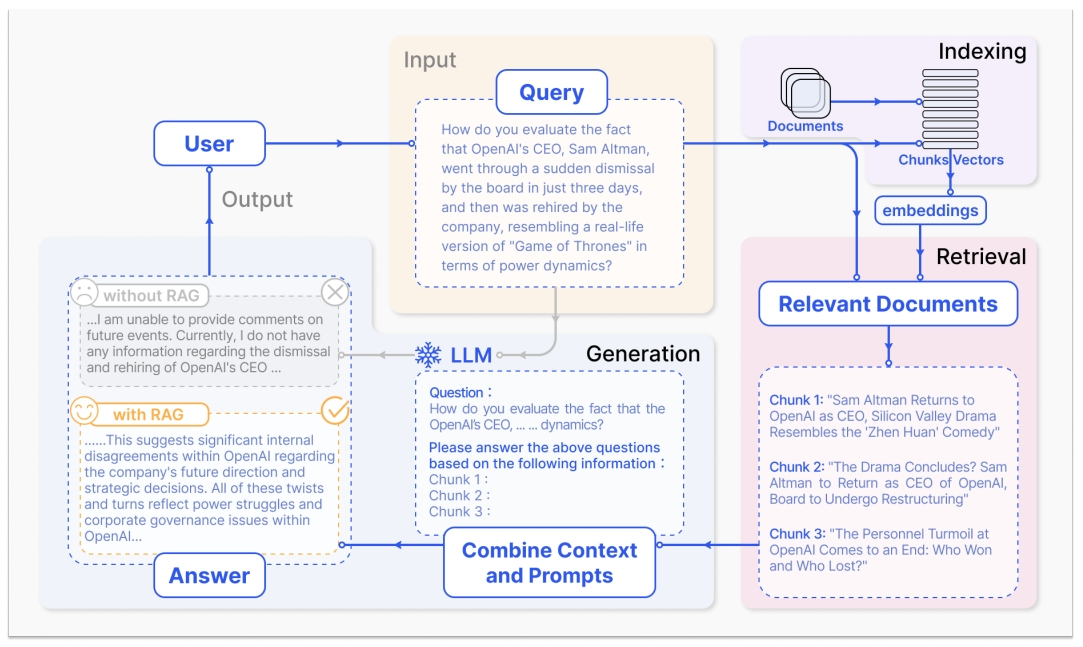
\includegraphics[width=1.0\textwidth]{image/rag.jpg}
  \caption[Alur \textit{Retrieval-Augmented Generation}]{Alur \textit{Retrieval-Augmented Generation} \parencite{gao2023rag}}
  \label{gambar:rag_workflow}
\end{figure}


% ==========================================
% 2.1.2 Hallucinations atau Konfabulasi pada Large Language Models
% ==========================================

\subsection{\textit{Hallucinations} atau Konfabulasi pada \textit{Large Language Models}}
\label{subsec:hallucinations-llm}

Konsep \textit{hallucination} pada awalnya berasal dari bidang psikologi, yang mengacu pada pengalaman perseptual tanpa adanya rangsangan eksternal atau persepsi yang menyimpang dari realitas. Dalam konteks \textit{Natural Language Processing} (NLP), halusinasi merujuk pada keluaran model bahasa besar (\textit{Large Language Model} atau LLM) yang tidak konsisten dengan fakta atau bahkan tidak masuk akal. Namun, beberapa peneliti menilai bahwa istilah \textit{hallucination} tidak sepenuhnya tepat karena memberikan kesan bahwa model memiliki persepsi sensorik sebagaimana manusia. Sebagai alternatif, istilah \textit{confabulation} dianggap lebih akurat, karena menggambarkan kecenderungan seseorang untuk "mengisi celah memori" dengan informasi yang tampak benar namun sebenarnya keliru, suatu analogi yang sesuai dengan perilaku LLM ketika menghasilkan keluaran yang salah namun tampak meyakinkan \parencite{math2024hallucination}.

Dalam praktiknya, istilah \textit{hallucination} masih lebih banyak digunakan dalam literatur akademik karena telah menjadi istilah baku untuk menggambarkan fenomena keluaran tidak faktual pada LLM. Secara umum, halusinasi dapat dibedakan menjadi dua kategori utama, yaitu:
\begin{enumerate}[a.]
  \item \textbf{Halusinasi intrinsik}, yaitu ketika keluaran model bertentangan dengan masukan atau konteks sumber. Contohnya, model memberikan angka yang berbeda dari data yang sebenarnya terdapat dalam teks masukan.
  \item \textbf{Halusinasi ekstrinsik}, yaitu ketika keluaran tidak dapat diverifikasi dari masukan namun mungkin benar jika dibandingkan dengan pengetahuan eksternal \parencite{math2024hallucination}.
\end{enumerate}

Klasifikasi yang lebih mendalam dikemukakan oleh Huang et al. (2023) dengan menambahkan dua dimensi tambahan: halusinasi \textbf{faktualitas} (\textit{factuality hallucination}) dan halusinasi \textbf{kefidelan} (\textit{faithfulness hallucination}). Halusinasi faktualitas terjadi ketika keluaran tidak sesuai dengan fakta dunia nyata, sedangkan halusinasi kefidelan terjadi ketika keluaran menyimpang dari instruksi pengguna, konteks, atau logika internal model.
Rawte et al. (2024) bahkan mengajukan dua variasi tambahan, yakni \textit{factual mirage} (jawaban salah terhadap pertanyaan yang benar) dan \textit{silver lining} (jawaban tampak benar terhadap pertanyaan yang salah) \parencite{math2024hallucination}.

Dalam konteks
\textit{Retrieval-Augmented Generation} (RAG), batasan pengetahuan internal LLM dapat dikompensasi dengan pengambilan informasi eksternal. Namun, halusinasi tetap dapat muncul ketika sumber hasil \textit{retrieval} mengandung data yang salah, sudah usang, atau tidak relevan. Misalnya, apabila dokumen hasil pencarian mengandung informasi yang keliru, maka model dapat menghasilkan \textit{factual hallucination}. Sebaliknya, jika kueri pengguna ambigu, maka sistem dapat salah menafsirkan konteks dan menghasilkan \textit{faithfulness hallucination} \parencite{math2024hallucination}.

\begin{longtable}{|p{2cm}|p{2.5cm}|p{3.5cm}|p{4cm}|}
\caption{Contoh berbagai jenis \textit{hallucination} pada \textit{Large Language Models (LLM)}}
\label{tbl:jenis_hallucination_baru} \\
\hline
\textbf{Jenis \textit{Hallucination}} &
\textbf{Contoh Pertanyaan / Instruksi} &
\textbf{Keluaran Model} &
\textbf{Penjelasan} \\
\hline
\endfirsthead

\caption[]{Contoh jenis - jenis \textit{hallucination} pada \textit{Large Language Models} (lanjutan)} \\
\hline
\textbf{Jenis \textit{Hallucination}} &
\textbf{Contoh Pertanyaan / Instruksi} &
\textbf{Keluaran Model} &
\textbf{Penjelasan} \\
\hline
\endhead

\hline
\multicolumn{4}{r}{\textit{Bersambung pada halaman berikutnya}} \\
\endfoot

\hline
\endlastfoot

% -------------------- isi tabel --------------------

\textbf{Halusinasi Intrinsik} &
"Laporan keuangan Perusahaan A menunjukkan arus kas operasi sebesar CNY 520 juta. Analisislah kondisi arus kas Perusahaan A." &
"Arus kas bersih dari aktivitas investasi sebesar CNY 380 juta." &
Keluaran model bertentangan dengan informasi numerik pada \textit{prompt}. Nilai yang dihasilkan tidak sesuai dengan angka yang diberikan, sehingga menunjukkan ketidakselarasan konteks internal terhadap data awal. \\ \hline

\textbf{Halusinasi Ekstrinsik} &
"Laporan keuangan Perusahaan A menunjukkan arus kas operasi sebesar CNY 520 juta. Analisislah kondisi arus kas Perusahaan A." &
"Peningkatan arus kas disebabkan oleh ekspansi ke pasar Asia Tenggara." &
Model menghasilkan penjelasan berbasis informasi eksternal yang tidak tercantum pada dokumen sumber. Secara linguistik dan logis jawaban tampak konsisten, namun tidak didukung konteks faktual pada data input. \\ \hline

\textbf{Halusinasi Faktualitas} &
"Sebutkan nama presiden Amerika Serikat saat ini." &
"Presiden Amerika Serikat saat ini adalah William Howard Taft." &
Keluaran model mengandung klaim faktual yang keliru. Nama pejabat publik yang disebutkan tidak merepresentasikan realitas politik aktual, menunjukkan kesalahan substansi meskipun format kalimat tersusun baik. \\ \hline

\textbf{Halusinasi Ketidakselarasan Tugas} &
"Terjemahkan: Who was the director of \textit{Avatar}?" &
"\textit{Avatar} disutradarai oleh James Cameron." &
Model tidak mengikuti instruksi utama yang diminta, yaitu melakukan penerjemahan. Model justru menjawab isi pertanyaan. Ketidaktaatan terhadap tujuan instruksi menunjukkan kegagalan pemahaman arah tugas. \\ \hline

\textbf{Factual Mirage} &
"Sir Arthur Conan Doyle adalah penulis seri Sherlock Holmes. Jelaskan penghargaan resmi yang diterimanya." &
"Arthur Conan Doyle menerima penghargaan 'Royal Detective Honor' dari Kerajaan Inggris." &
Model memproduksi entitas fiktif yang tampak kredibel dan relevan dengan konteks. Padahal, penghargaan tersebut tidak pernah ada. Fenomena ini mencerminkan pembentukan fakta semu yang sulit dibedakan dari informasi nyata. \\ \hline

\textbf{Silver Lining} &
"Mengapa Lin Daiyu mencabut pohon willow?" &
"Lin Daiyu mencabut pohon willow sebagai simbolisasi kesedihan mendalam atas nasib tragisnya." &
Model menjawab berdasarkan asumsi naratif dari teks yang diberikan, padahal tindakan yang menjadi premis dalam \textit{prompt} tidak pernah terjadi pada karya aslinya. Ketika dipaksa menerima pernyataan yang salah, model memvalidasi konteks fiktif dan mengembangkan narasi lanjutan. \\ \hline

\end{longtable}



Fenomena halusinasi pada LLM dapat disebabkan oleh tiga faktor utama:
\begin{enumerate}[a.]
  \item keterbatasan pengetahuan internal model akibat cakupan data pelatihan yang terbatas;
  \item ketidaksesuaian antara kueri pengguna dan hasil pencarian pada tahap \textit{retrieval};
  \item kesalahan integrasi atau interpretasi konteks eksternal pada tahap \textit{generation}.
\end{enumerate}

Dengan demikian, deteksi dan mitigasi halusinasi menjadi aspek penting dalam pengembangan sistem berbasis LLM, khususnya pada domain yang menuntut keakuratan dan kredibilitas tinggi seperti kesehatan, keuangan, serta pendidikan \parencite{math2024hallucination}.

Khusus pada domain biomedis, halusinasi pada sistem RAG tidak hanya dipengaruhi oleh keterbatasan model pada tahap \textit{generation}, tetapi juga oleh kegagalan \textit{retrieval} akibat penggunaan akronim yang tidak konsisten antara kueri pengguna dan dokumen ilmiah. Ketika istilah panjang pada kueri tidak cocok dengan akronim yang tertulis pada abstrak (\textit{vocabulary mismatch}), dokumen yang sebenarnya relevan gagal ditemukan, dan kekosongan konteks ini kemudian memicu model menghasilkan jawaban yang tidak \textit{grounded}. Oleh karena itu, mitigasi halusinasi pada domain biomedis perlu memperbaiki dua hal sekaligus, yaitu memastikan dokumen yang relevan berhasil ditemukan pada tahap \textit{retrieval} dan memastikan jawaban tetap setia pada dokumen tersebut pada tahap \textit{generation}.

% % ==========================================
% % 2.3 Deteksi Halusinasi Menggunakan LRP4RAG
% % ==========================================

% \section{Deteksi Halusinasi Menggunakan LRP4RAG}
% \label{sec:lrp4rag}

% Tugas Akhir terbaru oleh Hua dkk. (2025) memperkenalkan \textbf{LRP4RAG}, sebuah metode inovatif untuk mendeteksi halusinasi pada sistem \textit{Retrieval-Augmented Generation (RAG)} dengan memanfaatkan algoritma \textit{Layer-wise Relevance Propagation (LRP)} \parencite{lrp4rag2024}. Pendekatan ini berangkat dari premis bahwa hubungan antara konteks yang diambil dan keluaran model dapat dianalisis secara kuantitatif melalui distribusi relevansi antar lapisan pada arsitektur transformer. Dengan menelusuri kontribusi setiap token terhadap jawaban yang dihasilkan, metode ini mampu mengidentifikasi apakah suatu respons bersandar pada bukti kontekstual yang valid atau mengandung halusinasi.

% \textit{LRP4RAG} dibangun atas dua penyebab utama munculnya halusinasi pada sistem RAG, yaitu:
% \begin{enumerate}[1.]
%   \item \textbf{Konteks yang terlalu panjang}. Model sering kali gagal mengenali bagian informasi yang paling relevan dalam konteks yang sangat panjang. Fenomena ini dikenal sebagai masalah "\textit{lost in the middle}", di mana bagian tengah konteks cenderung diabaikan, sehingga menyebabkan keluaran yang tidak akurat.
%   \item \textbf{Ketidaksesuaian antara kata dan pikiran internal}. Model dapat mengekspresikan jawaban yang tampak benar secara eksplisit, tetapi secara implisit (melalui jejak relevansi internal) ternyata berlandaskan konteks yang keliru. Ketidaksesuaian antara "\textit{words}" (bukti eksplisit) dan "\textit{thoughts}" (bukti implisit) ini sering kali menjadi sumber utama halusinasi \parencite{lrp4rag2024}.
% \end{enumerate}

% Untuk mengatasi permasalahan tersebut, \textit{LRP4RAG} mengadaptasi algoritma \textit{Layer-wise Relevance Propagation} (LRP) agar sesuai dengan model \textit{transformer}. LRP menghitung seberapa besar kontribusi setiap neuron terhadap keluaran model dengan melacak aliran relevansi secara mundur dari lapisan keluaran menuju lapisan masukan. Dalam konteks RAG, proses ini memungkinkan analisis hubungan antara setiap token konteks dengan token jawaban yang dihasilkan.

% Secara garis besar, \textit{LRP4RAG} terdiri dari empat tahapan utama:
% \begin{enumerate}[1.]
%   \item \textbf{RAG Retrieval}: sistem mengambil potongan dokumen paling relevan sebagai konteks berdasarkan pertanyaan pengguna.
%   \item \textbf{LRP Forward}: selama proses generasi jawaban, model menyimpan gradien antar lapisan untuk setiap token.
%   \item \textbf{LRP Backward}: proses propagasi balik dilakukan untuk menghasilkan matriks relevansi yang memetakan kontribusi setiap token konteks terhadap jawaban.
%   \item \textbf{Deteksi Halusinasi}: tahap akhir untuk menentukan apakah keluaran model konsisten dengan konteks berdasarkan analisis relevansi dan keselarasan semantik antar bagian teks.
% \end{enumerate}

% Dua varian utama dikembangkan dalam kerangka \textit{LRP4RAG}:
% \begin{itemize}
%   \item \textbf{LRP4RAGClassifier}: mengubah matriks relevansi menjadi vektor fitur numerik yang mewakili tingkat keterkaitan antara konteks dan jawaban. Vektor ini kemudian dimasukkan ke dalam model klasifikasi biner seperti \textit{Support Vector Machine (SVM)}, \textit{Random Forest}, atau \textit{LSTM} untuk mendeteksi apakah jawaban mengandung halusinasi.
%   \item \textbf{LRP4RAGLLM}: metode tanpa pelatihan tambahan yang memanfaatkan kemampuan penalaran LLM untuk melakukan pemeriksaan konsistensi. Metode ini membandingkan keselarasan antara bukti implisit (bagian konteks dengan relevansi tertinggi dari hasil LRP) dan bukti eksplisit (bagian konteks yang diidentifikasi secara sadar oleh model melalui \textit{prompt}). Ketidaksesuaian antara keduanya menjadi indikasi adanya halusinasi \parencite{lrp4rag2024}.
% \end{itemize}

% Hasil eksperimen menunjukkan bahwa \textit{LRP4RAG} secara signifikan mengungguli sepuluh metode deteksi halusinasi terkini lainnya, termasuk \textit{SelfCheckGPT}, \textit{Semantic Entropy Probe (SEP)}, dan \textit{SAPLMA}. Pada pengujian terhadap dataset \textit{RAGTruth} dan \textit{Dolly-15k}, \textit{LRP4RAGLLM} meningkatkan akurasi sebesar 4,1\% hingga 5,1\% dibandingkan baseline terbaik sebelumnya. Selain itu, analisis relevansi pada tingkat token menunjukkan bahwa sampel dengan halusinasi memiliki korelasi konteks-jawaban yang lebih lemah dibandingkan sampel normal.

% Kelebihan utama \textit{LRP4RAG} terletak pada kemampuan interpretasinya: setiap nilai relevansi dapat ditelusuri kembali ke token sumber, sehingga model tidak hanya memberikan hasil deteksi, tetapi juga penjelasan mengapa suatu keluaran diklasifikasikan sebagai halusinasi. Meskipun \textit{LRP4RAGLLM} memiliki keunggulan dalam akurasi dan konsistensi semantik, varian \textit{LRP4RAGClassifier} menawarkan efisiensi komputasi yang lebih tinggi dan kemudahan penerapan pada sistem dengan sumber daya terbatas.

% Secara keseluruhan, \textit{LRP4RAG} memberikan kontribusi penting terhadap pengembangan sistem LLM yang lebih transparan dan dapat dipercaya. Dengan menggabungkan prinsip interpretabilitas aditif dan analisis relevansi lapisan, pendekatan ini membuka jalan baru dalam mendeteksi serta memahami penyebab halusinasi pada sistem \textit{Retrieval-Augmented Generation} \parencite{lrp4rag2024}.

% % ==========================================
% % 2.4 RAG-HAT: A Hallucination-Aware Tuning Pipeline
% % ==========================================

% \section{\textit{RAG-HAT: A Hallucination-Aware Tuning Pipeline}}
% \label{sec:raghat}

% Tugas Akhir oleh Song dkk. (2024) memperkenalkan \textbf{RAG-HAT} (\textit{Hallucination-Aware Tuning Pipeline for Large Language Models in Retrieval-Augmented Generation}), yaitu kerangka pelatihan yang dirancang untuk mengurangi halusinasi pada sistem \textit{Retrieval-Augmented Generation (RAG)} melalui proses penyesuaian preferensi berbasis kesadaran halusinasi \parencite{raghat2024}. Pendekatan ini berfokus pada penyetelan perilaku model agar dapat mendeteksi, menulis ulang, dan memitigasi konten yang terdeteksi sebagai halusinasi tanpa memerlukan model penghargaan eksplisit seperti pada \textit{reinforcement learning} tradisional.

% \textit{RAG-HAT} dikembangkan untuk menjawab dua permasalahan utama yang muncul dalam pendekatan mitigasi halusinasi konvensional:
% \begin{enumerate}[1.]
%   \item \textbf{Kesulitan membuat dataset preferensi halusinasi}. Dalam eksperimen sebelumnya (misalnya pada \textit{RAGTruth}), para anotator mengalami kesulitan menentukan jenis halusinasi mana yang lebih parah karena perbedaan persepsi dan subjektivitas dalam penilaian tingkat kesalahan.
%   \item \textbf{Ketidaktepatan dalam memperlakukan "tidak berhalusinasi" sebagai preferensi tunggal}. Menjadikan "bebas halusinasi" sebagai satu-satunya preferensi justru membuat model terlalu kaku dan berisiko menolak menjawab atau memberikan tanggapan terlalu defensif. Oleh sebab itu, \textit{RAG-HAT} memperkenalkan penyesuaian yang lebih alami terhadap preferensi ini, agar model dapat menyeimbangkan antara kehati-hatian dan keberanian menjawab \parencite{raghat2024}.
% \end{enumerate}

% Arsitektur \textit{RAG-HAT} dibangun atas tiga tahap utama, yaitu:

% \begin{enumerate}[1.]
%   \item \textbf{Deteksi} : model mengenali segmen keluaran yang mengandung konten tidak didukung bukti atau tidak konsisten dengan konteks hasil \textit{retrieval}.
% \end{enumerate}

% \begin{figure}[H]
%   \centering
%   \captionsetup{justification=centering}
%   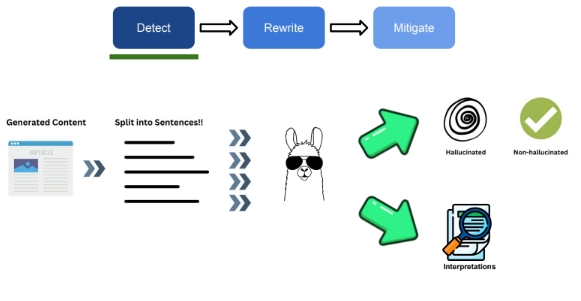
\includegraphics[width=0.85\textwidth]{image/raghat1.jpg}
%   \caption{Tahap Deteksi pada Arsitektur RAG-HAT}
%   \label{gambar:raghat_deteksi}
% \end{figure}

% \begin{enumerate}[2.]
%   \item \textbf{Penulisan ulang} (\textit{rewrite}) : bagian yang terdeteksi sebagai halusinasi digenerasi ulang berdasarkan konteks sumber dengan instruksi eksplisit untuk mempertahankan \textit{faithfulness}.
% \end{enumerate}

% \begin{figure}[H]
%   \centering
%   \captionsetup{justification=centering}
%   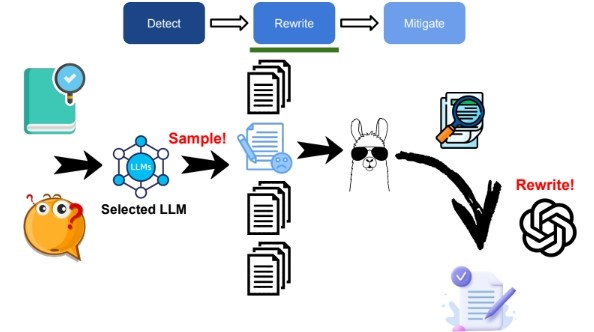
\includegraphics[width=0.85\textwidth]{image/raghat2.jpg}
%   \caption{Tahap Penulisan Ulang (\textit{Rewrite}) pada Arsitektur RAG-HAT}
%   \label{gambar:raghat_rewrite}
% \end{figure}

% \begin{enumerate}[3.]
%   \item \textbf{Mitigasi} : hasil akhir dievaluasi ulang untuk memastikan tidak terjadi penalti berlebihan (\textit{overly cautious penalization}) yang dapat mengurangi kelancaran atau keluwesan model dalam menjawab.
% \end{enumerate}

% \begin{figure}[H]
%   \centering
%   \captionsetup{justification=centering}
%   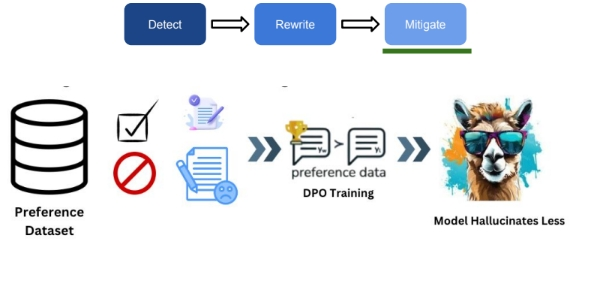
\includegraphics[width=0.85\textwidth]{image/raghat3.jpg}
%   \caption{Tahap Mitigasi pada Arsitektur RAG-HAT}
%   \label{gambar:raghat_mitigasi}
% \end{figure}


% Proses penyetelan preferensi pada \textit{RAG-HAT} menggunakan mekanisme \textit{Direct Performance Alignment (DPA)}, yang merupakan bentuk penyesuaian perilaku model tanpa memerlukan pelatihan model penghargaan terpisah seperti pada \textit{Reinforcement Learning with Human Feedback (RLHF)}. DPA memungkinkan penyesuaian langsung berdasarkan hasil keluaran yang lebih disukai tanpa memperkirakan fungsi penghargaan secara eksplisit. Hal ini menjadikan \textit{RAG-HAT} lebih efisien secara komputasi serta lebih mudah diimplementasikan dibanding pendekatan berbasis RLHF \parencite{raghat2024}.

% Keunggulan utama \textit{RAG-HAT} dibandingkan metode lain seperti \textit{SelfCheckGPT} atau \textit{LRP4RAG} adalah sifatnya yang \textbf{proaktif}. Alih-alih hanya mendeteksi kesalahan setelah respons dihasilkan, \textit{RAG-HAT} melakukan mitigasi secara terintegrasi dalam tahap generasi itu sendiri, sehingga mengurangi kemungkinan halusinasi sejak awal proses produksi teks. Pendekatan ini dapat dirangkum dalam prinsip \textbf{"Detect--Rewrite--Mitigate"}, yang menekankan daur adaptif antara deteksi dan koreksi untuk menjaga konsistensi keluaran terhadap konteks \parencite{raghat2024}.

% Selain itu, \textit{RAG-HAT} menerapkan strategi "\textit{defensive advice}" untuk menghindari penalti berlebihan yang dapat membuat model terlalu berhati-hati. Dengan demikian, model tetap mampu menghasilkan keluaran yang informatif namun terkendali secara faktual.

% Eksperimen menunjukkan bahwa \textit{RAG-HAT} mampu mengurangi tingkat halusinasi pada sistem RAG sebesar 6,3\% hingga 8,7\% dibandingkan baseline GPT-4 yang telah di-\textit{instruction-tuned}. Selain itu, model hasil penyetelan \textit{RAG-HAT} menunjukkan peningkatan pada metrik \textit{faithfulness} dan \textit{factual consistency} tanpa menurunkan kelancaran jawaban.

% Dengan mengintegrasikan proses deteksi, penulisan ulang, dan penyesuaian preferensi secara langsung dalam pipeline, \textit{RAG-HAT} menjadi salah satu pendekatan paling efektif dalam menyeimbangkan antara ketepatan faktual dan kemampuan generatif pada \textit{Large Language Models}. Pendekatan ini memperkuat arah tugas akhir ke depan untuk menghasilkan sistem RAG yang lebih \textit{hallucination-resilient} dan dapat dipercaya \parencite{raghat2024}.

% ==========================================
% 2.5 Mitigasi Halusinasi pada Retrieval-Augmented Generation
% ==========================================

\section{Mitigasi Halusinasi pada \textit{Retrieval-Augmented Generation}}
\label{sec:mitigasi_halusinasi}

Tinjauan oleh Math dkk.\ (2025) memberikan pemetaan komprehensif mengenai fenomena \textit{hallucination} pada \textit{Retrieval-Augmented Generation} (RAG), mulai dari sumber penyebab di setiap tahap \textit{pipeline} hingga teknik mitigasi yang telah diusulkan dalam literatur \parencite{math2024hallucination}. RAG sendiri dirancang untuk mengurangi ketergantungan LLM pada pengetahuan parametris dengan menambahkan konteks eksternal, tetapi dalam praktiknya sistem ini tetap rentan menghasilkan keluaran yang tidak akurat ketika terjadi kegagalan pada tahap \textit{retrieval} maupun \textit{generation}.

Secara garis besar, \textit{hallucination} pada RAG dikelompokkan ke dalam dua sumber utama: \textbf{\textit{retrieval failure}} dan \textbf{\textit{generation deficiency}}. \textit{Retrieval failure} muncul ketika sistem gagal menemukan atau memilih informasi yang relevan, misalnya karena kueri ambigu, pemeringkatan dokumen yang buruk, atau korpus yang berisi data usang. Sementara itu, \textit{generation deficiency} berkaitan dengan ketidakmampuan model untuk menyelaraskan jawaban dengan konteks yang sudah benar, misalnya akibat panjang konteks, konflik antar sumber, atau desain \textit{prompt} yang tidak tegas \parencite{math2024hallucination}.

\begin{figure}[H]
  \centering
  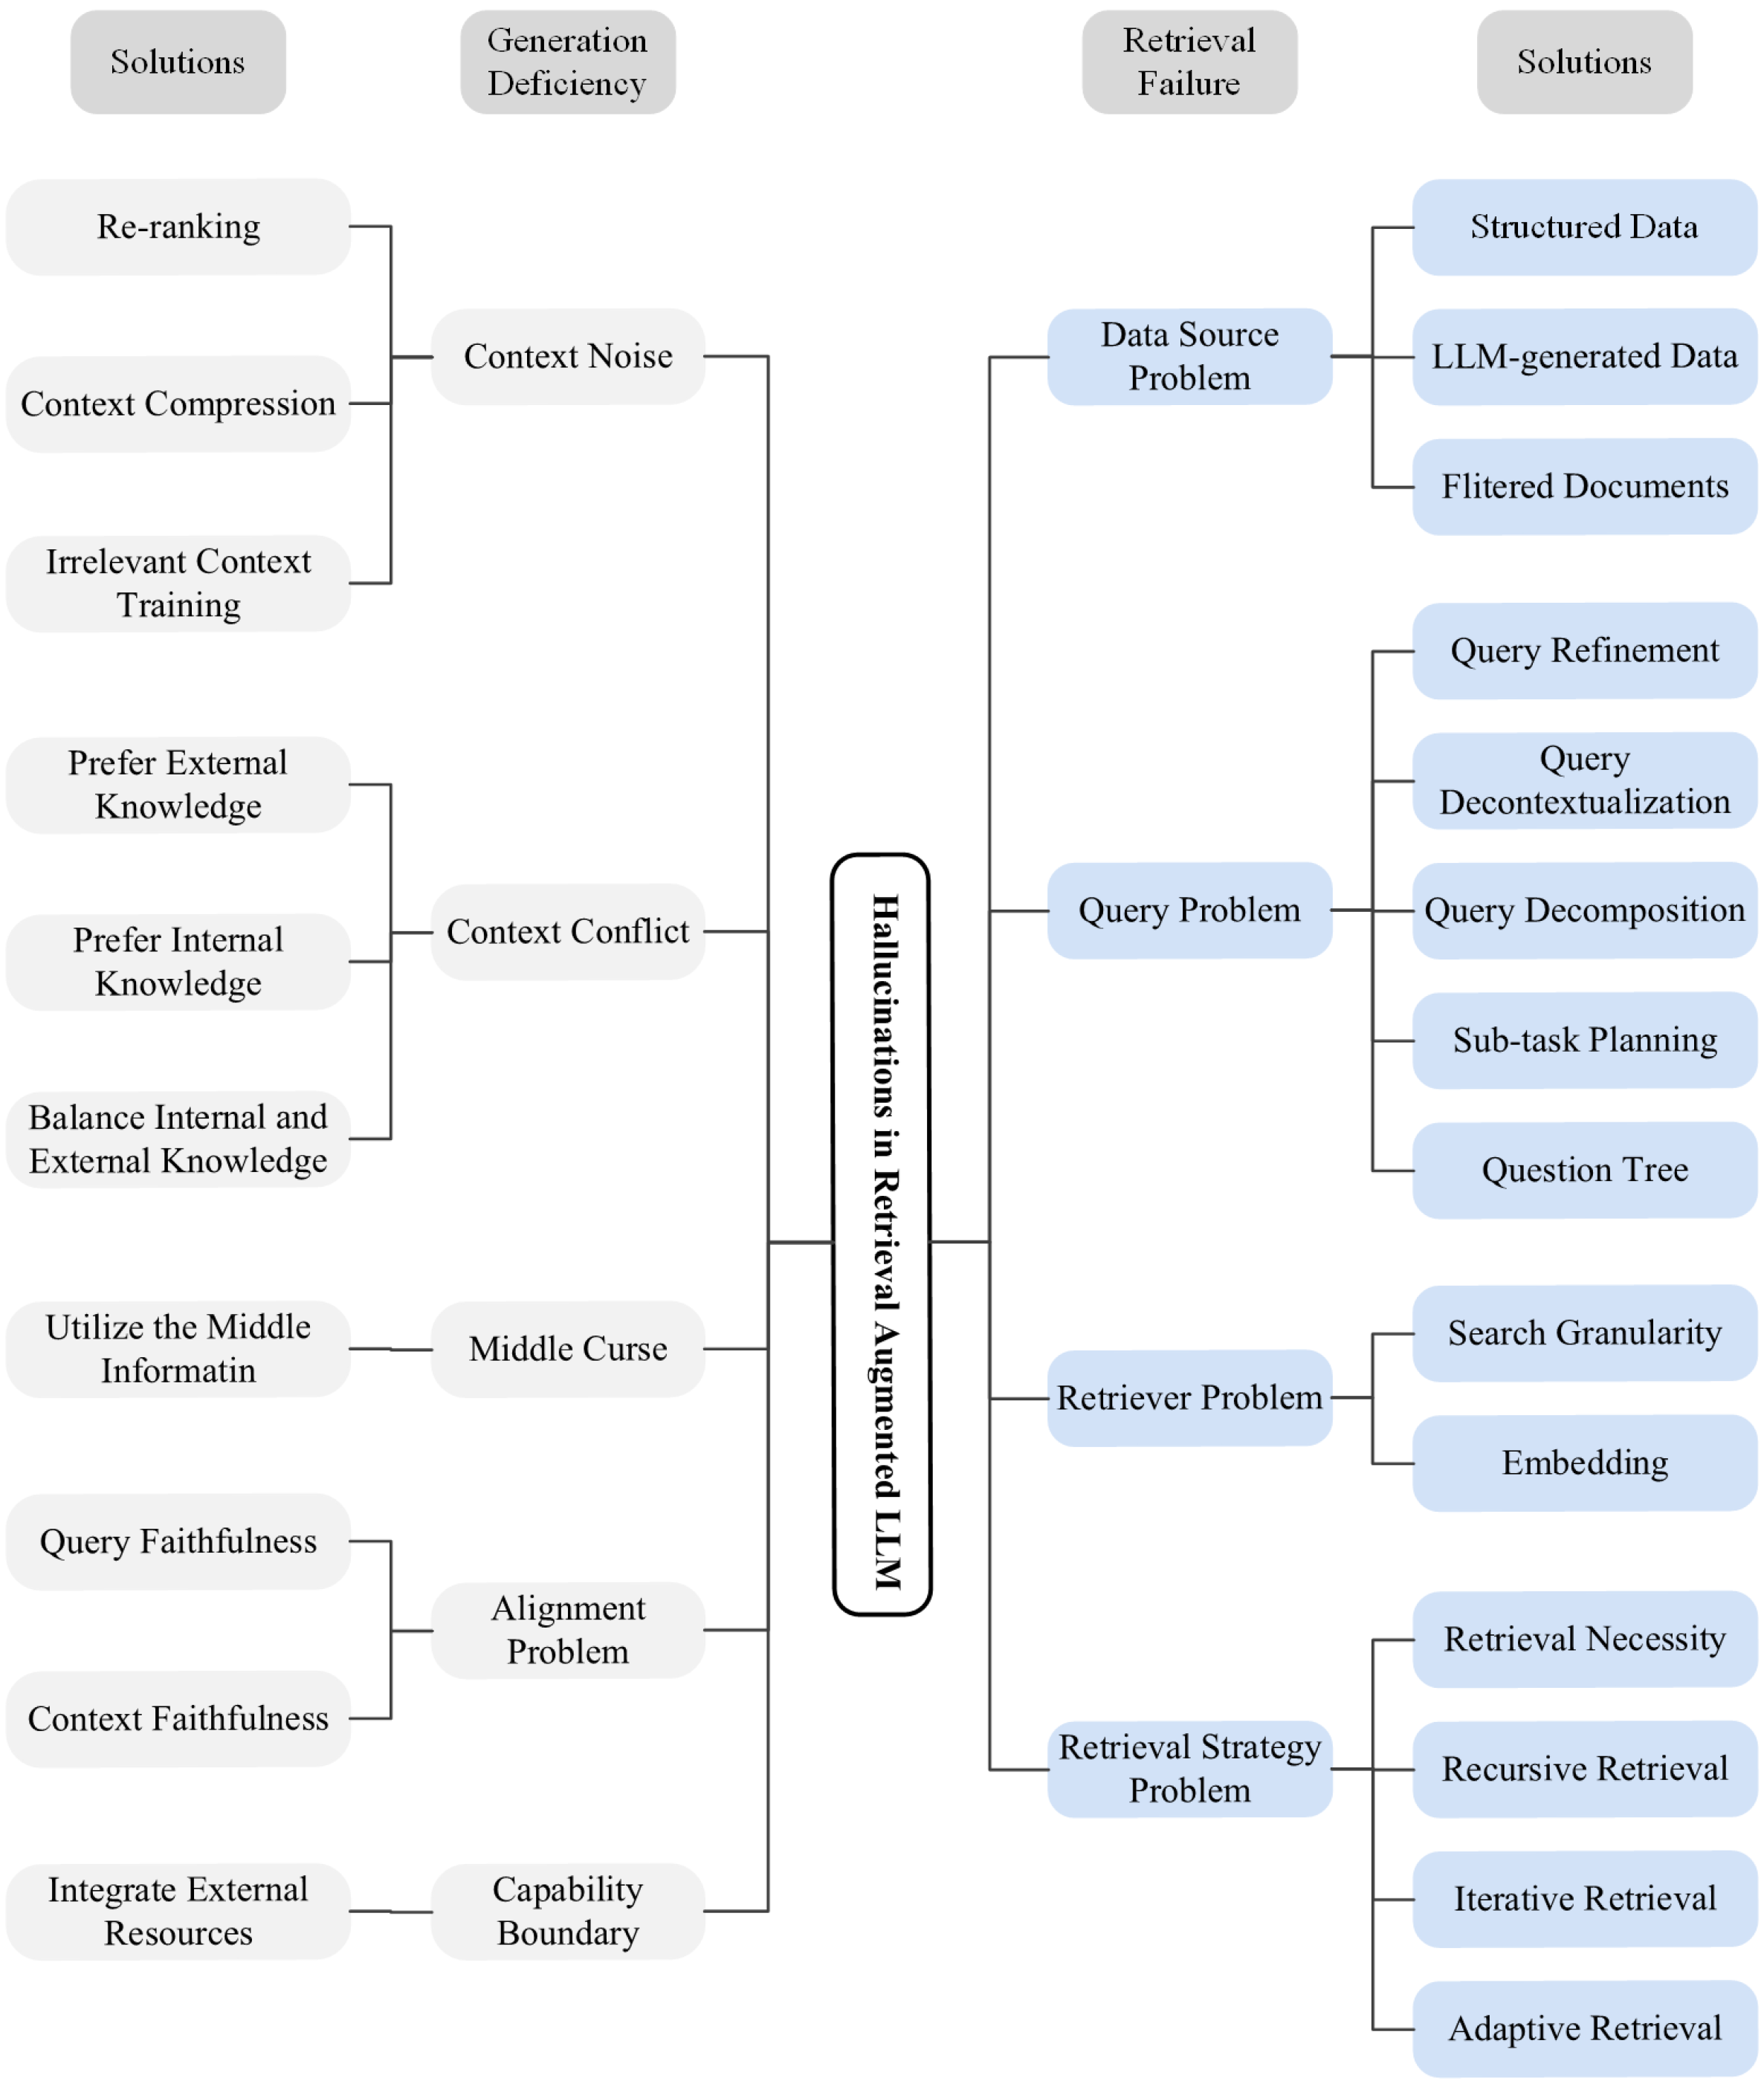
\includegraphics[width=0.95\textwidth]{image/causesofhallu.png}
  \caption[Penyebab dan solusi halusinasi pada RAG-LLM]{Penyebab dan solusi halusinasi pada RAG-LLM (\textcite{math2024hallucination}).}
  \label{fig:causes_hallucination_rag}
\end{figure}


Bagian ini menguraikan kerangka RAG yang dibahas oleh Math dkk.\ (2025), teknik mitigasi yang diusulkan pada setiap subtugas, serta ringkasan metrik dan dataset yang digunakan untuk mengevaluasi keberhasilan mitigasi tersebut, sebagaimana dirangkum pada publikasi tersebut.

% ------------------------------------------
% 2.5.1 Kerangka RAG dan Titik Munculnya Halusinasi
% ------------------------------------------

\subsection{Kerangka RAG dan Titik Munculnya \textit{Hallucination}}
\label{subsec:rag-framework-math}

Math dkk.\ memodelkan sistem RAG sebagai rangkaian subtugas yang tersebar di beberapa tahap utama \parencite{math2024hallucination}:

\begin{enumerate}[1.]
  \item \textbf{Pemahaman kueri} (\textit{query understanding})
  Sistem menafsirkan pertanyaan atau instruksi pengguna dan membentuk kueri yang akan digunakan pada modul \textit{retrieval}. Ambiguitas, ketidaklengkapan, atau pemilihan kata yang keliru pada tahap ini dapat berujung pada \textit{retrieval failure}.

  \item \textbf{Pengambilan dokumen} (\textit{document retrieval})
  Berdasarkan kueri, \textit{retriever} memilih dokumen atau potongan teks (\textit{passage}) yang dianggap paling relevan dari korpus. Kinerja yang buruk pada tahap ini menghasilkan konteks yang tidak relevan, tidak lengkap, atau bias.

  \item \textbf{Seleksi dan pemrosesan konteks} (\textit{context selection and processing})
  Sistem memilih subset konteks yang akan dimasukkan ke dalam \textit{prompt}, sering kali dengan melakukan pemotongan, pemeringkatan ulang, atau kompresi. Di sini dapat muncul masalah seperti konteks terlalu panjang, informasi penting terpotong, atau kebisingan yang tidak tersaring.

  \item \textbf{Integrasi pengetahuan} (\textit{knowledge integration})
  LLM menggabungkan pengetahuan parametris internal dengan konteks eksternal yang diambil melalui \textit{retrieval}. Konflik antara pengetahuan internal dan eksternal, atau kegagalan dalam mengutamakan bukti dari konteks, dapat memicu \textit{hallucination}.

  \item \textbf{Generasi jawaban} (\textit{answer generation})
  Pada tahap ini, model menghasilkan teks akhir yang akan diterima pengguna. Desain \textit{prompt}, strategi decoding, dan tidak adanya mekanisme verifikasi dapat membuat model memproduksi pernyataan yang tidak didukung dokumen.
\end{enumerate}

Dengan memetakan subtugas seperti di atas, Math dkk.\ menekankan bahwa mitigasi halusinasi tidak bisa hanya dilakukan dengan satu teknik pada satu tahap, melainkan memerlukan \textit{pipeline} yang secara eksplisit menangani sumber kesalahan di tahap \textit{retrieval} maupun \textit{generation}.

% ------------------------------------------
% 2.5.2 Mitigasi pada Tahap Retrieval
% ------------------------------------------

\subsection{Mitigasi Halusinasi pada Tahap \textit{Retrieval}}
\label{subsec:retrieval-mitigation}

Pada tahap \textit{retrieval}, halusinasi umumnya berasal dari kueri yang tidak representatif serta pemeringkatan dokumen yang tidak tepat. Math dkk.\ mengelompokkan teknik mitigasi utama sebagai berikut \parencite{math2024hallucination}.

\subsubsection{Perbaikan Kueri dan \textit{Query Rewriting}}

Jika kueri pengguna terlalu pendek, ambigu, atau mengandung istilah yang tidak spesifik, \textit{retriever} dapat mengembalikan dokumen yang tidak relevan. Untuk mengurangi masalah ini, beberapa studi mengusulkan:

\begin{itemize}
  \item \textbf{\textit{Query rewriting}} berbasis LLM, yaitu menulis ulang pertanyaan pengguna menjadi kueri yang lebih terstruktur, eksplisit, dan kaya konteks.
  \item \textbf{Ekspansi kueri} (\textit{query expansion}) dengan menambahkan sinonim, istilah teknis terkait, atau entitas yang relevan.
  \item \textbf{\textit{Decontextualization}}, yaitu mengubah pertanyaan yang bergantung pada konteks percakapan menjadi bentuk mandiri sehingga lebih mudah dicocokkan dengan dokumen.
\end{itemize}

Teknik-teknik ini bertujuan mengurangi \textit{retrieval failure} yang muncul semata-mata karena formulasi kueri yang kurang baik. Dalam konteks tugas akhir ini, modul \textit{query rewriting} dapat ditempatkan sebelum \textit{retriever} untuk memastikan bahwa kueri yang masuk ke tahap berikutnya sudah dioptimalkan.

\subsubsection{Peningkatan Kualitas \textit{Retriever} dan \textit{Reranking}}

Selain memperbaiki kueri, banyak penelitian fokus pada peningkatan kualitas \textit{retriever} itu sendiri. Pendekatan yang dibahas dalam tinjauan tersebut meliputi:

\begin{itemize}
  \item Penggunaan \textbf{\textit{dense retriever}} berbasis \textit{embedding}, yang menangkap kedekatan semantik di luar kecocokan kata kunci.
  \item \textbf{\textit{Hybrid retrieval}} yang menggabungkan metode klasik seperti BM25 dengan \textit{dense retriever} untuk menyeimbangkan presisi dan jangkauan.
  \item \textbf{\textit{Reranking}} dokumen menggunakan model yang lebih kuat (misalnya model \textit{cross-encoder}) untuk menilai kembali relevansi top-$k$ hasil awal.
\end{itemize}

\textit{Reranking} menjadi penting ketika \textit{retriever} bekerja pada skala besar: alih-alih mencoba mengoptimalkan seluruh daftar hasil, sistem fokus pada memeringkat ulang sejumlah kecil kandidat teratas. Dengan demikian, konteks yang akhirnya dimasukkan ke \textit{prompt} memiliki probabilitas lebih tinggi untuk benar-benar relevan, yang pada gilirannya mengurangi risiko \textit{hallucination} di tahap \textit{generation}.

\subsubsection{Seleksi dan Kompresi Konteks}

Masalah lain yang disorot adalah \textit{lost in the middle}, di mana LLM cenderung mengabaikan bagian tengah konteks yang panjang. Untuk mengatasi hal ini, beberapa teknik yang dibahas antara lain:

\begin{itemize}
  \item \textbf{Kompresi semantik} (\textit{semantic compression}), misalnya melalui model seperti \textit{LLMLingua}, yang merangkum konteks menjadi bentuk lebih ringkas namun tetap informatif.
  \item \textbf{Seleksi kontekstual} (\textit{selective context selection}), yaitu memilih hanya kalimat atau paragraf yang paling relevan terhadap pertanyaan.
  \item \textbf{\textit{Chunking} dan pengurutan adaptif}, di mana dokumen dipecah menjadi segmen-segmen kecil dan diurutkan ulang berdasarkan kedekatan dengan kueri.
\end{itemize}

Teknik seleksi dan kompresi ini menurunkan tingkat kebisingan pada konteks, sehingga model tidak terdorong membuat asumsi ketika berhadapan dengan informasi yang tidak relevan atau terlalu banyak.

% ------------------------------------------
% 2.5.3 Mitigasi pada Tahap Integrasi Pengetahuan
% ------------------------------------------

\subsection{Mitigasi pada Tahap Integrasi Pengetahuan}
\label{subsec:integration-mitigation}

Pada tahap integrasi pengetahuan, LLM harus menggabungkan pengetahuan internal dengan bukti eksternal. Math dkk.\ menyoroti beberapa tantangan utama: konflik antar sumber, konsistensi logika, dan pemilihan bukti yang tepat \parencite{math2024hallucination}.

Untuk mengurangi \textit{hallucination} pada tahap ini, beberapa pendekatan yang dibahas antara lain:

\begin{itemize}
  \item \textbf{Konsolidasi pengetahuan} (\textit{knowledge consolidation}), di mana sistem menyusun representasi terstruktur dari bukti sebelum generasi jawaban akhir.
  \item \textbf{Resolusi konflik} antar dokumen dengan meminta model mengidentifikasi perbedaan dan memilih bukti yang paling kredibel.
  \item \textbf{Mekanisme memori} (\textit{memory mechanisms}) yang menyimpan fakta penting dari konteks sehingga tidak hilang ketika model memproses konteks yang panjang.
\end{itemize}

Meskipun tugas akhir ini tidak secara langsung mengimplementasikan modul integrasi pengetahuan khusus, pemahaman terhadap tahap ini penting untuk menjelaskan bahwa mitigasi di tingkat \textit{retrieval} dan \textit{generation} perlu didesain agar selaras.

% ------------------------------------------
% 2.5.4 Mitigasi pada Tahap Generasi
% ------------------------------------------

\subsection{Mitigasi Halusinasi pada Tahap \textit{Generation}}
\label{subsec:generation-mitigation}

Pada tahap \textit{generation}, Math dkk.\ mengkaji berbagai teknik yang berfokus pada cara model menghasilkan dan memverifikasi jawaban \parencite{math2024hallucination}. Beberapa kategori utama adalah sebagai berikut.

\subsubsection{\textit{Prompt Engineering} dan Strategi Penalaran}

Berbagai teknik \textit{prompting} digunakan untuk memandu model agar lebih berhati-hati, antara lain:

\begin{itemize}
  \item \textbf{\textit{Chain-of-thought}} dan penalaran bertahap yang mendorong model menjelaskan langkah berpikirnya.
  \item \textbf{\textit{Vigilant prompting}} yang secara eksplisit menginstruksikan model untuk hanya menggunakan informasi dari konteks dan menyatakan ``tidak tahu'' jika bukti tidak memadai.
  \item \textbf{Teknik lanjutan} seperti \textit{ReAct}, CoVe, CoN, dan CoK yang memadukan penalaran, aksi, verifikasi, dan pengelolaan dokumen untuk menekan \textit{hallucination}.
\end{itemize}

Teknik-teknik ini tidak mengubah parameter model, tetapi mengatur perilaku generasi melalui desain \textit{prompt} yang cermat.

\subsubsection{Verifikasi Jawaban dan \textit{Active Detection}}

Selain mengarahkan proses generasi, banyak tugas akhir yang menambahkan lapisan verifikasi setelah jawaban dihasilkan. Contoh pendekatan yang dibahas dalam tinjauan tersebut meliputi:

\begin{itemize}
  \item \textbf{Pemeriksaan berbasis konsistensi}, seperti \textit{SelfCheckGPT}, yang membandingkan beberapa sampel generasi untuk menilai stabilitas klaim \parencite{selfcheckgpt2023}.
  \item \textbf{Verifikasi berbasis sumber}, misalnya dengan memformulasikan ulang jawaban menjadi serangkaian pertanyaan dan memeriksanya terhadap konteks \textit{retrieval}.
  \item \textbf{Deteksi segmen halusinatif}, di mana model atau klasifikator tambahan menandai kalimat atau frasa yang tidak didukung bukti, untuk kemudian ditulis ulang atau dihapus.
\end{itemize}

Pendekatan-pendekatan verifikasi tersebut menggambarkan bahwa keluaran model masih dapat diperiksa ulang melalui lapisan tambahan setelah generasi sebagai salah satu arah mitigasi halusinasi pada sistem RAG. Pada tugas akhir ini, fokus mitigasi diarahkan pada tahap praproses dokumen, \textit{retrieval}, dan pemilihan konteks, sehingga lapisan verifikasi pascagenerasi berada di luar cakupan dan dibahas hanya sebagai konteks pustaka.



% ==========================================
% 2.3 Ekspansi Akronim Dokumen pada Sistem RAG
% ==========================================

\section{Ekspansi Akronim Dokumen pada Sistem RAG}
\label{sec:ekspansi-akronim-rag}

Salah satu sumber utama kegagalan pada sistem RAG adalah ketidakcocokan kosakata (\textit{vocabulary mismatch}) antara kueri pengguna dan dokumen pada korpus, yaitu kondisi ketika makna semantik antara keduanya sebenarnya sama namun bentuk istilahnya berbeda. Untuk mengatasi hal ini, salah satu strategi yang banyak diadopsi adalah memperkaya isi setiap dokumen sebelum diindeks, sehingga setiap \textit{chunk} mengandung istilah yang lebih beragam dan lebih dekat dengan gaya kueri pengguna. Strategi ini dikenal sebagai \textit{document expansion} atau \textit{document enrichment}.

Strategi pengayaan dokumen telah terbukti efektif pada berbagai domain. Pada domain finansial, \textcite{fintechrag2025} dan \textcite{financialmeta2025} menyuntik akronim domain-spesifik, sinonim, serta metadata terstruktur ke dokumen sebelum diindeks, dan melaporkan peningkatan akurasi \textit{retrieval} yang konsisten dibandingkan \textit{baseline} BM25 maupun \textit{dense retrieval} tunggal. Pada domain enterprise yang lebih umum, \textcite{enterprisekg2025} mengusulkan kerangka sistematis yang memanfaatkan model bahasa besar untuk membangkitkan metadata terenrichi (kata kunci, entitas, akronim, sinonim) pada tiap \textit{chunk}, dengan hasil peningkatan retrieval hingga sepuluh poin persentase pada korpus internal perusahaan. Pendekatan serupa pada level enrichment per-chunk juga diusulkan oleh \textcite{mdkeychunker2025} yang menggabungkan ekstraksi kata kunci, ringkasan, dan pertanyaan hipotetis melalui satu pemanggilan LLM. Pola yang konsisten lintas-domain ini menegaskan bahwa pengayaan dokumen pada tahap \textit{indexing} merupakan strategi yang dapat digeneralisasi dan menjadi salah satu fondasi penting pada sistem RAG modern.

% ==========================================
% 2.4 BM25 sebagai Algoritma Retrieval Klasik
% ==========================================

\section{BM25 sebagai Algoritma \textit{Retrieval} Klasik}
\label{sec:bm25-teori}

BM25 (\textit{Best Matching 25}) adalah algoritma \textit{retrieval} berbasis statistik yang dikembangkan oleh Robertson dan kolega pada awal tahun 1990-an sebagai penyempurnaan dari skema TF-IDF. Algoritma ini memberi peringkat dokumen terhadap suatu kueri berdasarkan tiga prinsip utama, yaitu seberapa sering istilah kueri muncul pada dokumen (\textit{term frequency}), seberapa langka istilah tersebut pada keseluruhan korpus (\textit{inverse document frequency}), serta seberapa panjang dokumen tersebut dibandingkan rata-rata panjang dokumen pada korpus. Tiga prinsip ini memastikan dokumen yang lebih banyak memuat istilah kueri yang langka dan tidak terlalu panjang akan menempati peringkat lebih atas dibandingkan dokumen yang sekadar panjang dan kebetulan mengulang istilah umum.

Skor BM25 untuk pasangan dokumen $D$ dan kueri $Q$ dirumuskan sebagai berikut.

\begin{equation}
\label{eq:bm25}
\text{BM25}(D, Q) = \sum_{q \in Q} \text{IDF}(q) \cdot \frac{f(q, D) \cdot (k_1 + 1)}{f(q, D) + k_1 \cdot \left(1 - b + b \cdot \dfrac{|D|}{\text{avgdl}}\right)}
\end{equation}

Pada Persamaan~\ref{eq:bm25}, $f(q, D)$ menyatakan jumlah kemunculan istilah $q$ pada dokumen $D$, $|D|$ adalah panjang dokumen $D$ dalam jumlah kata, dan $\text{avgdl}$ adalah rata-rata panjang dokumen pada korpus. Sementara itu, $\text{IDF}(q)$ adalah komponen \textit{inverse document frequency} yang dihitung sebagai berikut.

\begin{equation}
\label{eq:bm25-idf}
\text{IDF}(q) = \ln \left( \dfrac{N - n(q) + 0{,}5}{n(q) + 0{,}5} + 1 \right)
\end{equation}

Pada Persamaan~\ref{eq:bm25-idf}, $N$ adalah jumlah total dokumen pada korpus dan $n(q)$ adalah jumlah dokumen yang memuat istilah $q$ minimal sekali. Persamaan ini memberikan bobot yang lebih besar pada istilah langka, sehingga kemunculan istilah seperti ``hyperbaric'' lebih berkontribusi terhadap skor dibandingkan istilah umum seperti ``patient'' atau ``study''.

Dua parameter $k_1$ dan $b$ pada Persamaan~\ref{eq:bm25} mengatur perilaku algoritma. Parameter $k_1$ mengendalikan tingkat saturasi \textit{term frequency}, yaitu seberapa cepat tambahan kemunculan istilah berhenti memberi kontribusi tambahan terhadap skor; nilai standar yang sering dipakai pada literatur adalah $k_1 = 1{,}5$. Parameter $b$ mengendalikan tingkat normalisasi panjang dokumen, dengan nilai standar $b = 0{,}75$ yang menyeimbangkan antara dokumen panjang dan pendek tanpa menghukum keduanya secara berlebihan. Kombinasi kedua parameter ini memberi BM25 keunggulan dibandingkan TF-IDF murni karena tidak terlalu sensitif terhadap panjang dokumen maupun pengulangan istilah yang berlebihan.

% ==========================================
% 2.5 Dense Retrieval dan Pencarian Berbasis Vektor
% ==========================================

\section{\textit{Dense Retrieval} dan Pencarian Berbasis Vektor}
\label{sec:dense-teori}

\textit{Dense retrieval} adalah pendekatan pencarian dokumen yang merepresentasikan baik kueri maupun dokumen sebagai vektor numerik berdimensi tinggi, lalu menghitung kemiripan antara dua vektor sebagai dasar peringkat. Berbeda dengan BM25 yang hanya mencocokkan kata kunci, \textit{dense retrieval} memanfaatkan kemampuan model bahasa untuk menangkap makna semantik teks, sehingga dokumen yang menggunakan istilah berbeda tetapi maknanya mirip dengan kueri tetap dapat ditemukan. Sebagai contoh, kueri yang menyebut ``\textit{physical activity}'' dapat menemukan dokumen yang menulis ``\textit{exercise}'' atau ``\textit{aerobic training}'', selama ketiga istilah tersebut berdekatan posisinya pada ruang vektor.

Setiap teks pada \textit{dense retrieval} diubah menjadi vektor melalui model \textit{embedding}, yaitu jaringan saraf yang telah dilatih agar pasangan teks dengan makna mirip menghasilkan vektor yang berdekatan, sedangkan pasangan teks dengan makna berbeda menghasilkan vektor yang berjauhan \parencite{reimers2019sbert}. Model \textit{embedding} modern umumnya berbasis arsitektur \textit{transformer} dan menghasilkan vektor berdimensi antara 256 hingga 1.536, tergantung ukuran dan tujuan model. Dimensi yang tinggi memungkinkan model menangkap nuansa makna yang lebih halus, namun juga menuntut kapasitas penyimpanan dan komputasi yang lebih besar.

Kemiripan antara vektor kueri $\vec{q}$ dan vektor dokumen $\vec{d}$ dihitung menggunakan \textit{cosine similarity}, yang mengukur sudut antara kedua vektor pada ruang berdimensi tinggi. Rumusnya adalah sebagai berikut.

\begin{equation}
\label{eq:cosine-similarity}
\text{cosine}(\vec{q}, \vec{d}) = \dfrac{\vec{q} \cdot \vec{d}}{\|\vec{q}\| \cdot \|\vec{d}\|}
\end{equation}

Pada Persamaan~\ref{eq:cosine-similarity}, $\vec{q} \cdot \vec{d}$ adalah \textit{dot product} antara kedua vektor, sedangkan $\|\vec{q}\|$ dan $\|\vec{d}\|$ adalah norma Euclidean dari masing-masing vektor. Nilai \textit{cosine similarity} berada pada rentang $[-1, 1]$, dengan nilai mendekati satu menandakan kemiripan makna yang tinggi, nilai mendekati nol menandakan tidak ada hubungan, dan nilai negatif menandakan makna yang bertolak belakang. Pada konteks pencarian dokumen, hanya dokumen dengan skor kemiripan tertinggi yang dipilih sebagai kandidat.

Keunggulan \textit{dense retrieval} dibandingkan BM25 terletak pada kemampuannya menangani parafrasa, sinonim, dan terminologi yang berbeda namun bermakna serupa. Pada sisi lain, \textit{dense retrieval} cenderung lemah pada pencocokan istilah teknis yang sangat spesifik (misalnya nama obat, gen, atau akronim langka) karena model \textit{embedding} mungkin belum cukup mengenali kosakata domain tersebut. Karakteristik ini menjadi alasan utama banyak sistem RAG modern memilih pendekatan \textit{hybrid retrieval} yang menggabungkan keunggulan kedua metode.

% ==========================================
% 2.6 Query Rewriting untuk Mitigasi Halusinasi pada RAG
% ==========================================

\section{\textit{Query Rewriting} untuk Mitigasi Halusinasi pada RAG}
\label{sec:queryrewriting}

Salah satu penyebab paling umum dari halusinasi dalam sistem \textit{Retrieval-Augmented Generation} (RAG) adalah kegagalan pada tahap \textit{retrieval}, terutama ketika kueri pengguna bersifat pendek, ambigu, atau tidak memiliki kata kunci yang sesuai dengan struktur dokumen dalam korpus. Untuk mengatasi kelemahan ini, Ma dkk.\ (2023) mengusulkan pendekatan \textbf{\textit{Query Rewriting for Retrieval-Augmented Large Language Models}}, yaitu teknik untuk mentransformasikan kueri mentah pengguna menjadi bentuk kueri baru yang lebih jelas, lebih informatif, dan lebih mudah dicocokkan oleh \textit{retriever} \parencite{ma2023queryrewriting}.

Pendekatan ini bekerja dengan memanfaatkan kemampuan \textit{Large Language Models} dalam menafsirkan maksud pengguna secara lebih mendalam, kemudian menghasilkan ulang kueri dalam bentuk yang kaya konteks. Tujuannya bukan sekadar memperpanjang kueri, melainkan:
\begin{enumerate}[1.]
  \item mengekspansi istilah penting yang tersirat,
  \item menambahkan kata kunci domain yang relevan,
  \item mendisambiguasi istilah atau objek yang memiliki lebih dari satu makna,
  \item menghilangkan ketidakjelasan linguistik,
  \item menyelaraskan format kueri dengan gaya penulisan korpus rujukan.
\end{enumerate}



Ma dkk.\ menunjukkan bahwa \textit{retriever} tradisional seperti BM25 atau Dense Passage Retrieval sering kali gagal menemukan dokumen yang benar ketika kueri terlalu pendek atau tidak selaras dengan distribusi bahasa pada korpus. Dengan memperbaiki bentuk kueri melalui proses \textit{rewriting}, sistem RAG dapat meningkatkan \textbf{recall} dokumen relevan secara signifikan, sehingga mengurangi risiko halusinasi pada tahap generasi karena model tidak perlu "mengarang" informasi untuk mengisi kekosongan konteks.

Secara teknis, pendekatan ini membingkai \textit{query rewriting} sebagai fungsi:
\[
q' = \text{LLM\_rewrite}(q),
\]
di mana $q$ adalah kueri awal pengguna, dan $q'$ adalah kueri terstruktur yang dihasilkan LLM. Kueri baru tersebut kemudian digunakan oleh \textit{retriever} untuk mendapatkan konteks:
\[
C = \text{Retriever}(q').
\]

\subsubsection*{Contoh Transformasi Kueri}
Berikut beberapa contoh hasil transformasi kueri menggunakan \textit{query rewriting}:

\begin{itemize}
  \item \textbf{Kueri awal:} ``How do I keep my plants alive while I'm on holiday?''

        \textbf{Kueri baru:} ``What are the best methods for ensuring my indoor and outdoor plants remain healthy and watered during a vacation?''

  \item \textbf{Kueri awal:} ``Which country had the most athletes in the Olympic parade?''

        \textbf{Kueri baru:} ``Which country had the largest number of athletes participating in the most recent Olympic opening ceremony parade?''

  \item \textbf{Kueri awal:} ``Why were there concerns about the Seine?''

        \textbf{Kueri baru:} ``What specific issues or concerns have arisen regarding the Seine River, such as pollution, flooding, or ecological impacts?''
\end{itemize}

Berdasarkan eksperimen dalam Ma dkk.\ (2023), teknik ini memberikan keuntungan berikut:
\begin{itemize}
  \item \textbf{Peningkatan relevansi konteks} melalui kueri yang lebih kaya informasi.
  \item \textbf{Penurunan \textit{retrieval failure}}, khususnya pada kueri pendek.
  \item \textbf{Peningkatan \textit{faithfulness}} jawaban karena LLM memperoleh konteks yang lebih akurat.
\end{itemize}

Dalam konteks ini, \textit{query rewriting} berfungsi sebagai \textbf{mekanisme mitigasi pada tahap retrieval}. Dengan mengolah ulang kueri pengguna sebelum proses pencarian dokumen, sistem RAG menjadi lebih stabil dan lebih tahan terhadap halusinasi baik intrinsik maupun ekstrinsik.



% ==========================================
% 2.X Reranking Konteks untuk Mengurangi Kebisingan
% ==========================================

\section{\textit{Context Reranking} untuk Mengurangi Kebisingan}
\label{sec:context-reranking}

Pada sistem \textit{Retrieval-Augmented Generation} (RAG), tahap \textit{retrieval} sering menghasilkan sekumpulan potongan dokumen (\textit{chunk}) yang tidak hanya relevan, tetapi juga mengandung informasi yang berulang, terlalu umum, atau bahkan tidak terkait dengan maksud kueri. Kondisi ini dikenal sebagai \textit{konteks berisik} dan dapat mendorong \textit{Large Language Model} (LLM) untuk melakukan \textit{hallucination}, karena model berusaha menyintesis jawaban dari bukti yang sebagian tidak tepat sasaran.

Gambar~\ref{fig:context-reranking-flow} mengilustrasikan posisi \textit{context reranking} pada alur RAG. Setelah kueri dipakai untuk menarik sejumlah dokumen kandidat (\textit{top-k}) dari basis data vektor melalui \textit{semantic search}, sebuah modul \textit{reranker} menilai ulang relevansi tiap dokumen terhadap kueri, lalu menyusun ulang urutannya sehingga dokumen yang paling relevan menempati peringkat teratas sebelum diteruskan ke tahap \textit{generation} \parencite{chitika2025reranking}.

\begin{figure}[H]
  \centering
  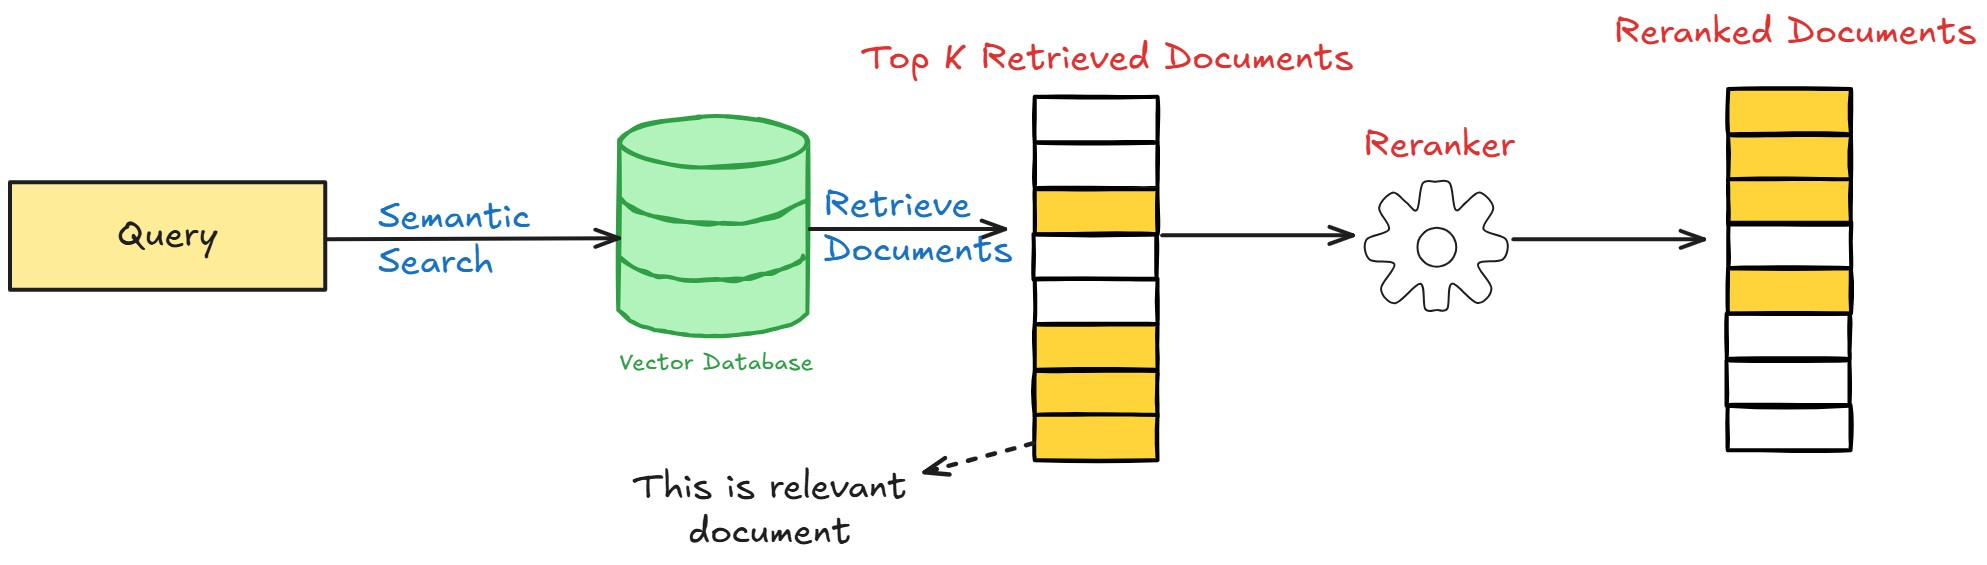
\includegraphics[width=0.95\textwidth]{image/context-rerankingflow.jpg}
  \caption[Alur kerja \textit{context reranking} pada sistem RAG]{Alur kerja \textit{context reranking} pada sistem RAG \parencite{chitika2025reranking}}
  \label{fig:context-reranking-flow}
\end{figure}

Ma dkk.\ mengkaji masalah ini pada skenario kueri yang bersifat \textit{multi-faceted}, yaitu ketika satu kueri pengguna memuat beberapa aspek atau \textit{sub-intent} sekaligus, misalnya dimensi produk, atribut kualitas, dan preferensi pengguna. Dalam kasus seperti ini, \textit{retriever} standar (misalnya \textit{BM25} atau \textit{dense retriever}) cenderung mengembalikan \textit{top-k} dokumen yang hanya menangkap sebagian aspek kueri dan mencampurkannya dengan dokumen yang relevansinya lemah.

Untuk mengurangi kebisingan dan meningkatkan kualitas konteks yang dikonsumsi oleh LLM, Ma dkk.\ mengusulkan modul \textit{context reranking}. Alih-alih langsung mengirim semua hasil \textit{retrieval} ke model generatif, sistem terlebih dahulu menerapkan tahap seleksi ulang (\textit{reranking}) terhadap \textit{top-k} kandidat. Secara garis besar, prosesnya meliputi:

\begin{enumerate}[1.]
  \item \textbf{Pengambilan kandidat awal} \\
  \textit{Retriever} menghasilkan \textit{top-k} potongan dokumen berdasarkan kemiripan awal terhadap kueri, misalnya dengan \textit{BM25}, \textit{dense retrieval}, atau \textit{vector database}. Hasil pada tahap ini masih berpotensi berisik dan tidak seimbang antar aspek kueri.

  \item \textbf{Penghitungan skor relevansi semantik} \\
  Setiap \textit{chunk} kandidat diberi skor relevansi terhadap representasi kueri yang diperkaya, tidak hanya berdasarkan kecocokan leksikal, tetapi juga kesesuaian semantik terhadap berbagai aspek kueri \parencite{craft2023richresponses}. Hal ini penting untuk menangkap bagian kueri yang bersifat \textit{multi-faceted}.

  \item \textbf{\textit{Multi-facet scoring} dan penalti kebisingan} \\
  Modul \textit{reranker} mengombinasikan beberapa komponen skor, antara lain: relevansi inti terhadap kueri, cakupan atribut atau aspek kueri, serta penalti untuk \textit{chunk} yang terlalu umum, redundant, atau tidak spesifik. Dengan cara ini, \textit{chunk} yang hanya mengandung informasi generik atau keluar dari konteks akan ditempatkan di peringkat bawah.

  \item \textbf{Pemilihan \textit{top-m} konteks terpilih} \\
  Berdasarkan skor komposit, sistem memilih \textit{top-m} \textit{chunk} terbaik sebagai konteks akhir yang akan diberikan kepada LLM. Nilai $m$ biasanya lebih kecil daripada $k$ sehingga konteks menjadi lebih ringkas, fokus, dan relevan.

  \item \textbf{Generasi jawaban berbasis konteks yang telah disaring} \\
  LLM kemudian menghasilkan jawaban dengan mengandalkan \textit{top-m} konteks terpilih tersebut. Karena kebisingan berkurang dan sudut pandang kueri tercakup dengan lebih seimbang, kecenderungan \textit{hallucination} dapat ditekan.
\end{enumerate}

Pendekatan \textit{context reranking} ini relevan karena berfokus pada deteksi dan mitigasi \textit{hallucination} pada sistem RAG. Pada tahap \textit{retrieval}, modul \textit{reranker} berperan sebagai filter kualitas yang memastikan hanya konteks yang paling relevan dan informatif yang diteruskan ke model generatif. Dengan demikian, \textit{hallucination} yang disebabkan oleh \textit{retrieval failure} berupa pemilihan dokumen yang salah atau berisik dapat dikurangi sebelum memasuki tahap \textit{generation} \parencite{math2024hallucination,craft2023richresponses}.

% ==========================================
% 2.X Active Detection untuk Mitigasi Halusinasi
% ==========================================

\section{\textit{Active Detection} untuk Mitigasi \textit{Hallucination}}
\label{sec:active-detection}

Varshney dkk.\ (2023) mengusulkan pendekatan \textit{active detection} sebagai mekanisme deteksi dan mitigasi \textit{hallucination} secara langsung selama proses generasi, bukan setelah teks sepenuhnya dihasilkan. Ide utamanya adalah bahwa \textit{Large Language Model} (LLM) menunjukkan pola tertentu ketika berada pada kondisi berisiko tinggi menghasilkan \textit{hallucination}, terutama ketika model menghasilkan token dengan tingkat kepercayaan rendah. Dengan melakukan pemeriksaan terhadap bagian yang memiliki \textit{low-confidence}, sistem dapat menghentikan proses generasi sementara dan memicu langkah verifikasi atau koreksi sebelum melanjutkan \parencite{varshney2023stitch}.

Pendekatan ini sangat relevan dalam konteks tugas akhir mengenai deteksi dan mitigasi \textit{hallucination} pada sistem \textit{Retrieval-Augmented Generation} (RAG), karena banyak \textit{hallucination} muncul pada bagian tertentu dari keluaran model, terutama ketika konteks eksternal kurang kuat atau ambigu.

\subsection{Prinsip Dasar \textit{Active Detection}}

Metode \textit{active detection} berangkat dari dua pengamatan kunci:

\begin{enumerate}[1.]
    \item \textbf{Token berisiko tinggi biasanya memiliki probabilitas rendah}.
    Model cenderung berada pada kondisi tidak pasti ketika menemukan konteks yang tidak jelas, dan hal ini tercermin melalui distribusi probabilitas token yang melebar. Token yang dipilih pada kondisi ini berpotensi menyebabkan \textit{hallucination}.

    \item \textbf{Verifikasi lokal dapat mencegah kesalahan global}.
    Dengan menghentikan generasi pada momen ketidakpastian dan melakukan pemeriksaan tambahan, sistem mampu memperbaiki kesalahan sebelum menjadi bagian dari keluaran akhir.
\end{enumerate}

\subsection{Alur Kerja \textit{Active Detection}}

Berdasarkan Varshney dkk.\ (2023), proses \textit{active detection} mencakup tiga langkah utama:

\begin{enumerate}[1.]
    \item \textbf{Identifikasi token berisiko rendah kepercayaan}
    Model memantau setiap langkah generasi dan menghitung nilai probabilitas token yang dihasilkan. Jika nilai tersebut berada di bawah ambang tertentu, sistem menandai posisi tersebut sebagai titik risiko.

    \item \textbf{Validasi token yang ditandai}
    Untuk token yang ditandai, sistem menjalankan proses verifikasi, misalnya melalui:
    \begin{itemize}
        \item \textit{self-consistency check}, yaitu model diminta menghasilkan beberapa alternatif untuk menilai kestabilan prediksi,
        \item \textit{entailment check} jika konteks tersedia,
        \item pembandingan semantik antara kandidat token dan konteks sumber.
    \end{itemize}

    \item \textbf{Koreksi sebelum melanjutkan generasi}
    Jika token berisiko dianggap tidak valid atau tidak didukung oleh konteks, model memilih alternatif token dengan probabilitas yang lebih tinggi atau mengulang prediksi. Dengan cara ini, kesalahan dicegah sebelum berkembang menjadi \textit{hallucination} yang lebih besar.
\end{enumerate}

\subsection{Kelebihan Metode \textit{Active Detection}}

Pendekatan ini menawarkan beberapa manfaat penting:

\begin{itemize}
    \item \textbf{Mitigasi proaktif}.
    Berbeda dengan metode pascagenerasi, \textit{active detection} mencegah \textit{hallucination} saat proses generasi berlangsung.

    \item \textbf{Tidak memerlukan model verifikator besar}.
    Seluruh proses berjalan dengan memanfaatkan informasi internal model, terutama distribusi probabilitas token.

    \item \textbf{Dapat dikombinasikan dengan RAG}.
    Dalam sistem RAG, metode ini dapat melengkapi pendekatan lain seperti \textit{context reranking} atau \textit{query rewriting}, sehingga mitigasi dapat dilakukan baik pada sisi \textit{retrieval} maupun pada saat generasi \parencite{math2024hallucination}.
\end{itemize}

\subsection{Keterbatasan}

Walaupun efektif, \textit{active detection} memiliki beberapa keterbatasan:

\begin{itemize}
    \item \textbf{Membutuhkan akses probabilitas token}.
    Pendekatan ini hanya dapat diterapkan pada model yang menyediakan \textit{logits} atau probabilitas token, sehingga tidak berlaku untuk model \textit{closed-source} tertentu.

    \item \textbf{Penentuan ambang yang sensitif}.
    Ambang probabilitas terlalu rendah gagal mendeteksi kesalahan, sedangkan ambang terlalu tinggi menyebabkan verifikasi berlebihan yang meningkatkan latensi.

    \item \textbf{Tidak selalu menangkap halusinasi semantik kompleks}.
    Token dengan probabilitas tinggi pun dapat menghasilkan klaim salah jika konteks \textit{retrieval} tidak relevan.
\end{itemize}


% % % ==========================================
% % % 2.2 Dataset RAGTruth (2025)
% % % ==========================================
% \section{Dataset RAGTruth (2025)}
% \label{sec:ragtruth}

% Untuk memahami dan mengukur fenomena \textit{hallucination} pada sistem \textit{Retrieval-Augmented Generation (RAG)}, diperlukan dataset dengan anotasi yang eksplisit terhadap kesalahan faktual dan ketidaksetiaan (\textit{unfaithfulness}) keluaran model. Salah satu dataset paling komprehensif yang dikembangkan untuk tujuan ini adalah \textbf{RAGTruth}, yang diperkenalkan oleh Niu et al. (2025) \parencite{ragtruth2025}. Dataset ini dirancang untuk memberikan dasar evaluasi yang lebih objektif terhadap fenomena halusinasi pada sistem berbasis LLM dengan pendekatan \textit{retrieval}.

% \textit{RAGTruth} menggabungkan tiga kategori tugas utama yang mencerminkan aplikasi nyata dari sistem berbasis RAG, yaitu:
% \begin{enumerate}[1.]
%   \item \textbf{Ulasan produk} (\textit{product review summarization}), yang mengevaluasi kemampuan model dalam menghasilkan ringkasan dari ulasan pengguna berdasarkan korpus yang diambil;
%   \item \textbf{Dialog berpengetahuan} (\textit{knowledge-grounded dialogue}), yang menilai sejauh mana model mampu menjaga kesetiaan terhadap konteks dokumen ketika melakukan percakapan;
%   \item \textbf{Pertanyaan berbasis dokumen} (\textit{document-based question answering}), yang menilai kemampuan model menjawab pertanyaan faktual berdasarkan teks sumber yang diambil melalui \textit{retriever}.
% \end{enumerate}

% Setiap sampel dalam dataset \textit{RAGTruth} terdiri dari:
% \begin{enumerate}[1.]
%   \item \textbf{Konteks sumber} (hasil \textit{retrieval});
%   \item \textbf{Keluaran model} (\textit{LLM output});
%   \item \textbf{Anotasi manual} pada tingkat kalimat dan token yang menandai segmen teks yang mengandung halusinasi, baik dari sisi fakta maupun kesetiaan \parencite{ragtruth2025}.
% \end{enumerate}


% Anotasi ini memungkinkan analisis kuantitatif terhadap dua dimensi kesalahan utama:
% \begin{enumerate}[a.]
%   \item \textbf{Faktualitas} : mengukur sejauh mana pernyataan model sesuai dengan fakta yang ada dalam dokumen sumber;
%   \item \textbf{Kefidelan} : menilai konsistensi keluaran terhadap konteks atau instruksi pengguna.
% \end{enumerate}

% Dataset \textit{RAGTruth} menandai kemajuan penting karena merupakan salah satu dataset pertama yang menyediakan anotasi pada level token secara manual untuk mendeteksi halusinasi. Ukuran dan keragaman datanya memungkinkan pelatihan serta pengujian model deteksi halusinasi berbasis \textit{supervised learning}, maupun pengujian metrik otomatis seperti \textit{BERTScore}, \textit{QAFactEval}, dan \textit{GPTScore}.

% Selain itu, \textit{RAGTruth} mengintegrasikan keluaran dari beberapa model besar, termasuk GPT-4, Claude, LLaMA-2, dan Falcon, sehingga hasil analisisnya bersifat lintas-model. Pendekatan ini memberi pandangan yang lebih menyeluruh tentang perbedaan perilaku halusinasi antar model dan interaksinya dengan sumber \textit{retrieval} \parencite{ragtruth2025}.

% Tabel~\ref{tbl:ragtruth_comparison} berikut memberikan ringkasan perbandingan antara dataset \textit{RAGTruth} dengan dataset deteksi halusinasi lainnya.

% \begin{table}[H]
% \centering
% \caption{Perbandingan dataset deteksi halusinasi berbasis RAG}
% \label{tbl:ragtruth_comparison}
% \begin{tabular}{|p{3.5cm}|p{3cm}|p{3cm}|p{4cm}|}
% \hline
% \textbf{Dataset} & \textbf{Jenis Tugas} & \textbf{Tingkat Anotasi} & \textbf{Keterangan Utama} \\ \hline
% \textbf{RAGTruth (2025)} &
% Ringkasan, Dialog, QA &
% Kalimat dan Token &
% Anotasi manual detail; mencakup model GPT, Claude, LLaMA, dan Falcon. \\ \hline
% \textbf{TRUE (2023)} &
% Ringkasan dan QA &
% Kalimat &
% Berbasis teks generik tanpa \textit{retrieval}; menilai kesalahan faktual umum. \\ \hline
% \textbf{FActScore (2023)} &
% QA dan Penjelasan &
% Kalimat &
% Mengukur \textit{faithfulness} berdasarkan fakta yang diklaim terhadap sumber. \\ \hline
% \textbf{QAFactEval (2022)} &
% QA &
% Kalimat &
% Metrik otomatis; tidak menyediakan anotasi manual. \\ \hline
% \end{tabular}
% \end{table}

% \textit{RAGTruth} tidak hanya berguna untuk evaluasi kinerja model generatif, tetapi juga untuk pengembangan algoritma mitigasi halusinasi. Misalnya, dengan memanfaatkan anotasi \textit{token-level}, model dapat dilatih untuk mendeteksi bagian keluaran yang tidak didukung bukti, lalu memperbaikinya menggunakan konteks tambahan melalui mekanisme \textit{re-ranking} atau \textit{self-consistency checking}.

% Secara keseluruhan, \textit{RAGTruth} memberikan kontribusi penting terhadap upaya standarisasi pengukuran halusinasi pada sistem RAG. Dengan cakupan domain yang luas dan anotasi yang presisi, dataset ini menjadi tolok ukur utama untuk tugas akhir deteksi dan mitigasi halusinasi pada \textit{Large Language Models} modern \parencite{ragtruth2025}.


% % ==========================================
% % 2.6 SelfCheckGPT: Deteksi Halusinasi Tanpa Sumber Eksternal
% % ==========================================

% \section{SelfCheckGPT: Deteksi Halusinasi Tanpa Sumber Eksternal}
% \label{sec:selfcheckgpt}

% \textbf{SelfCheckGPT} diperkenalkan sebagai pendekatan \textit{zero-resource} dan \textit{black-box} untuk mendeteksi \textit{hallucination} pada keluaran \textit{Large Language Models} (LLM) tanpa memerlukan data pelatihan khusus, model verifikator terpisah, ataupun korpus rujukan eksternal \parencite{selfcheckgpt2023}. Intuisi utamanya adalah memanfaatkan \textit{self-consistency}: jika suatu pernyataan benar dan stabil, maka beberapa sampel generasi yang dihasilkan dengan \textit{stochastic sampling} (misalnya pengaturan \textit{temperature} $>0$) cenderung saling bersepakat; sebaliknya, pernyataan halusinator akan menunjukkan ketidakselarasan antarsampel.

% Secara ringkas, prosedur \textit{SelfCheckGPT} meliputi:
% \begin{enumerate}[1.]
%   \item \textbf{Pembangkitan multi-sampel} (\textit{stochastic generations}) :model menghasilkan beberapa respons alternatif atas \textit{prompt} yang sama.
%   \item \textbf{Ekstraksi klaim/kalimat} :keluaran awal diurai menjadi klaim/kalimat kandidat untuk dicek.
%   \item \textbf{Pemeriksaan konsistensi} :setiap klaim dibandingkan dengan himpunan sampel alternatif menggunakan gabungan ukuran kesepakatan (\textit{overlap} leksikal), kesemestaan semantik (misalnya \textit{embedding similarity}), dan/atau pengujian \textit{entailment} berbasis \textit{Natural Language Inference (NLI)}.
%   \item \textbf{Skoring kehalusan} :derajat ketidakselarasan antarsampel dirangkum menjadi skor risiko \textit{hallucination} pada level kalimat atau keluaran.
% \end{enumerate}

% Karena bersifat \textit{black-box}, \textit{SelfCheckGPT} tidak mengakses probabilitas token internal dan tidak mengubah parameter model, cocok untuk skenario produksi yang membatasi akses model. Dalam pengujian pada berbagai \textit{benchmark} (misalnya \textit{question answering} dan \textit{summarization}), pendekatan ini menunjukkan kemampuan deteksi \textit{hallucination} yang kompetitif terhadap metrik berbasis probabilitas maupun metode verifikasi yang memerlukan \textit{retrieval} \parencite{selfcheckgpt2023}.

% % ------------------------------------------
% % 2.6.1 Kelebihan dan Keterbatasan
% % ------------------------------------------

% \subsection{Kelebihan dan Keterbatasan}
% \label{subsec:selfcheckgpt-advantages}

% \textit{SelfCheckGPT} menawarkan sejumlah kelebihan:
% \begin{enumerate}[a.]
%   \item \textbf{Tanpa sumber eksternal} :tidak membutuhkan dokumen rujukan atau \textit{knowledge base}; murni mengandalkan variansi generasi model.
%   \item \textbf{Model-agnostic dan \textit{deployment-friendly}} :dapat diterapkan pada model tertutup (\textit{closed-source}) dan mudah diintegrasikan ke dalam \textit{pipeline} yang sudah ada.
%   \item \textbf{Granularitas fleksibel} :dapat memberikan penilaian pada level kalimat/klaim maupun keseluruhan jawaban.
% \end{enumerate}

% Adapun keterbatasan utama:
% \begin{enumerate}[i.]
%   \item \textbf{Biaya komputasi} :memerlukan beberapa kali generasi ulang (\textit{multi-sampling}), sehingga latensi dan biaya inferensi meningkat.
%   \item \textbf{Ambiguitas tanpa bukti} :tanpa bukti eksternal, ketidakselarasan tidak selalu berarti salah (misalnya untuk topik yang memang ambigu atau terbuka).
%   \item \textbf{Sensitif terhadap strategi sampling} :kualitas deteksi dipengaruhi oleh pengaturan \textit{temperature}, jumlah sampel, dan bentuk \textit{prompting}.
% \end{enumerate}

% % ------------------------------------------
% % 2.6.2 Posisi terhadap RAG dan Metode Lain
% % ------------------------------------------

% \subsection{Posisi terhadap RAG dan Metode Lain}
% \label{subsec:selfcheckgpt-position}

% Dalam konteks \textit{Retrieval-Augmented Generation (RAG)}, \textit{SelfCheckGPT} dapat dipakai sebagai \textit{fallback} ketika bukti eksternal terbatas atau berisik, atau sebagai \textit{layer} verifikasi tambahan setelah pemeriksaan berbasis sumber (\textit{source-grounded checking}).

% Berbeda dengan \textit{LRP4RAG} yang memetakan relevansi token secara interpretable atau \textit{RAG-HAT} yang melakukan mitigasi proaktif selama proses generasi, \textit{SelfCheckGPT} lebih menitikberatkan pada deteksi pascagenerasi berbasis konsistensi antarsampel.

% Kombinasi \textit{SelfCheckGPT} (deteksi \textit{black-box} tanpa sumber) dengan evaluasi berbasis sumber (misalnya \textit{RAGTruth}) dan mitigasi terarah (misalnya \textit{RAG-HAT}) dapat menghasilkan \textit{pipeline} yang seimbang antara cakupan, akurasi, dan biaya.


% ==========================================
% 2.7 Prompt Engineering untuk Reduksi Hallucination
% ==========================================

\section{\textit{Prompt Engineering} untuk Reduksi \textit{Hallucination}}
\label{sec:prompt-reduce-hallucination}

Selain arsitektur model dan kualitas data, perancangan \textit{prompt} juga berperan besar dalam memicu maupun mengurangi \textit{hallucination} pada LLM. Studi survei oleh Sahoo dkk.\ (2024) menunjukkan bahwa \textit{prompt engineering} tidak hanya berfungsi sebagai antarmuka instruksi, tetapi juga sebagai mekanisme pengendali perilaku model, termasuk dalam mengarahkan model agar lebih berhati-hati terhadap fakta dan sumber informasi \parencite{sahoo2024prompt}.

Secara umum, teknik \textit{prompting} untuk mengurangi \textit{hallucination} dapat dikelompokkan ke dalam beberapa pendekatan: (i) memperkaya konteks dengan informasi yang relevan melalui \textit{Retrieval-Augmented Generation} (RAG), (ii) menggabungkan penalaran dan aksi secara eksplisit seperti pada \textit{ReAct}, (iii) menambahkan tahapan verifikasi terstruktur seperti pada \textit{Chain-of-Verification (CoVe)}, (iv) mengelola dokumen hasil \textit{retrieval} yang berisik seperti pada \textit{Chain-of-Note (CoN)}, dan (v) mengintegrasikan pengetahuan secara bertahap seperti pada \textit{Chain-of-Knowledge (CoK)} \parencite{sahoo2024prompt}. Pendekatan-pendekatan ini memanfaatkan \textit{prompt} bukan hanya sebagai instruksi tunggal, melainkan sebagai rangkaian langkah yang membantu model menelusuri bukti, memeriksa konsistensi, dan menolak menjawab ketika informasi tidak memadai.

Pada RAG, \textit{prompt} dirancang untuk memasukkan potongan dokumen hasil \textit{retrieval} ke dalam instruksi sehingga model terdorong mendasarkan jawabannya pada konteks eksternal, bukan hanya pada memori parametrik. \textit{Prompt} yang menekankan frasa seperti ``gunakan hanya informasi dari konteks berikut'' atau ``kutip sumber yang mendukung jawaban'' terbukti meningkatkan \textit{faithfulness} karena model diarahkan untuk menghasilkan jawaban berbasis bukti \parencite{lewis2020retrieval,ragtruth2025}.

Pendekatan \textit{ReAct} (\textit{Reasoning and Acting}) memadukan langkah penalaran (\textit{thought}) dan tindakan (\textit{action}) di dalam \textit{prompt}. Alih-alih langsung menghasilkan jawaban akhir, LLM diminta untuk menuliskan jejak penalaran singkat, memutuskan kapan perlu memanggil alat eksternal (misalnya API pencarian), lalu memperbarui rencana berdasarkan informasi baru \parencite{yao2022react}. Pola \textit{prompt} seperti ``\textit{Thought:} ...'', ``\textit{Action: Search[...]}'', dan ``\textit{Observation:} ...'' membantu model menyadari keterbatasannya dan mengurangi kecenderungan mengarang informasi.

\textit{Chain-of-Verification (CoVe)} menambahkan tahap verifikasi eksplisit. \textit{Prompt} meminta model untuk: (i) menghasilkan jawaban awal, (ii) menyusun daftar pertanyaan verifikasi, (iii) menjawab pertanyaan tersebut secara independen, dan (iv) merevisi jawaban sesuai hasil verifikasi \parencite{dhuliawala2024cove}. Pendekatan ini meniru metode pemeriksaan ulang yang dilakukan manusia, sehingga efektif dalam mengurangi \textit{hallucination} faktual.

\textit{Chain-of-Note (CoN)} berfokus pada pengelolaan dokumen hasil \textit{retrieval} yang berisik. Melalui \textit{prompt} yang meminta model menyoroti poin penting, mengabaikan dokumen tidak relevan, serta menandai ketidakpastian, CoN menjadikan model lebih selektif terhadap bukti yang digunakan \parencite{yu2024con}.

Sementara itu, \textit{Chain-of-Knowledge (CoK)} memecah masalah kompleks menjadi langkah penalaran bertahap. Mulai dari persiapan konteks, pengumpulan bukti dari sumber heterogen, hingga integrasi dan koreksi progresif. \textit{Prompt} mengarahkan model untuk tidak langsung melompat ke jawaban akhir, melainkan membangun penalaran yang terstruktur \parencite{li2023cok}. CoK mengurangi \textit{hallucination} yang muncul akibat penalaran terburu-buru dan tidak ter-grounding.

Secara keseluruhan, literatur menegaskan bahwa \textit{prompt} yang terstruktur, eksplisit, dan berlapis lebih mampu mengurangi \textit{hallucination} dibandingkan \textit{prompt} sederhana yang hanya berupa satu instruksi. Dengan demikian, \textit{prompt engineering} merupakan komponen penting dalam rancangan sistem LLM yang andal dan \textit{faithful}.

% ------------------------------------------
% 2.7.1 Zero-shot dan Few-shot Prompting
% ------------------------------------------

\subsection{\textit{Zero-shot} dan \textit{few-shot prompting}}
\label{subsec:zerofewshot}

Dua paradigma mendasar dalam \textit{prompting} adalah \textit{zero-shot prompting} dan \textit{few-shot prompting}. Keduanya menjadi fondasi bagi teknik lanjutan seperti \textit{ReAct}, CoVe, CoN, dan CoK.

\textit{Zero-shot prompting} adalah skenario ketika LLM diminta menyelesaikan suatu tugas hanya berdasarkan instruksi natural tanpa diberikan contoh format sebelumnya. Misalnya instruksi: ``Jelaskan perbedaan antara \textit{AHA} dan \textit{BHA} untuk kulit berjerawat.'' Model mengandalkan kemampuan generalisasi dari \textit{pre-training} dan \textit{instruction tuning}. Pendekatan ini fleksibel, tetapi rentan memicu \textit{hallucination} jika instruksinya ambigu atau tidak menyertakan batasan konteks.

Sebaliknya, \textit{few-shot prompting} memberikan beberapa contoh tugas--jawaban sebelum model diminta menjawab pertanyaan baru. Contohnya, dua atau tiga contoh penjelasan bahan aktif \textit{skincare} berbasis jurnal dapat disertakan dalam \textit{prompt}. Model kemudian belajar dari pola tersebut melalui mekanisme \textit{in-context learning} \parencite{zhao2023survey}. Ketika contoh yang diberikan \textit{faithful}, teknik ini dapat mengurangi \textit{hallucination} karena model meniru gaya jawaban yang berbasis bukti.

Dalam konteks mitigasi \textit{hallucination}, kedua paradigma ini sering dipadukan dengan instruksi tambahan. Misalnya, \textit{zero-shot} dilengkapi klausa: ``jawablah hanya berdasarkan konteks berikut dan nyatakan jika informasi tidak tersedia.'' Sedangkan \textit{few-shot} dapat menambahkan contoh jawaban yang menunjukkan bagaimana model harus menolak menjawab ketika bukti tidak memadai. Dengan demikian, baik \textit{zero-shot} maupun \textit{few-shot prompting} tidak hanya mengarahkan model memahami tugas, tetapi juga mengelola ketidakpastian dan mencegah \textit{hallucination}.

% ==========================================
% 2.8 Kerangka Kerja Evaluasi Sistem RAG
% ==========================================

\section{Kerangka Kerja Evaluasi Sistem \textit{Retrieval-Augmented Generation} (RAG)}
\label{sec:kerangka-evaluasi-rag}

Pengembangan sistem \textit{Retrieval-Augmented Generation} (RAG) memerlukan metode \textit{tuning} yang tepat karena kinerjanya dipengaruhi oleh berbagai komponen seperti model \textit{retriever}, model bahasa (\textit{language model}), rancangan \textit{prompt}, serta parameter konfigurasi lainnya. Oleh karena itu, evaluasi sistem RAG yang terotomasi menjadi hal yang penting dalam memastikan keluaran model yang akurat, relevan, dan berlandaskan bukti \parencite{es2024ragas}.

Evaluasi sistem RAG dapat dilakukan pada dua tingkat. Pertama, evaluasi pada tahap \textit{retrieval} yang berfokus pada kualitas dokumen yang berhasil ditemukan oleh \textit{retriever}. Kedua, evaluasi pada tahap \textit{generation} yang berfokus pada kualitas jawaban akhir yang dihasilkan oleh \textit{Large Language Model} berdasarkan konteks tersebut. Pada tugas akhir ini, evaluasi tahap \textit{retrieval} menggunakan tiga metrik konvensional yaitu \textit{Recall@k}, \textit{Mean Average Precision} (MAP@k), dan \textit{Normalized Discounted Cumulative Gain} (nDCG@k), sedangkan evaluasi tahap \textit{generation} menggunakan kerangka kerja \textit{Retrieval-Augmented Generation Assessment} (RAGAS).

% =====================================================
\subsection{Metrik Evaluasi \textit{Retrieval}}
\label{subsec:metrik-retrieval}

Metrik evaluasi \textit{retrieval} mengukur kualitas pencarian dokumen pada korpus, mulai dari kelengkapan dokumen relevan yang ditemukan hingga kualitas peringkatnya. Pada tugas akhir ini digunakan tiga metrik utama yang lazim dipakai dalam literatur \textit{Information Retrieval} dan RAG \parencite{ma2023queryrewriting, cormack2009reciprocal, lewis2020retrieval}.

\subsubsection{\textit{Recall@k}}

\textit{Recall@k} mengukur kelengkapan informasi yang berhasil di-\textit{retrieve} oleh sistem, yaitu proporsi dokumen relevan pada korpus yang berhasil muncul dalam $k$ dokumen teratas hasil pencarian. Metrik ini cocok untuk mengevaluasi seberapa baik sistem menangkap seluruh dokumen relevan yang tersedia, terutama pada tugas yang membutuhkan konteks lengkap seperti \textit{question answering} berbasis RAG. Rumus \textit{Recall@k} ditulis sebagai berikut:

\begin{equation}
\text{Recall@}k = \frac{|\{d \in R_q\} \cap \{d_1, d_2, \dots, d_k\}|}{|R_q|}
\end{equation}

dengan $R_q$ adalah himpunan seluruh dokumen relevan untuk \textit{query} $q$ pada korpus, dan $\{d_1, d_2, \dots, d_k\}$ adalah $k$ dokumen teratas yang dikembalikan oleh sistem \textit{retrieval}. Nilai \textit{Recall@k} berkisar antara 0 dan 1, di mana nilai 1 menunjukkan bahwa seluruh dokumen relevan berhasil ter-\textit{retrieve} dalam $k$ teratas.

\subsubsection{\textit{Mean Average Precision} (MAP@k)}

\textit{Mean Average Precision} mengukur kualitas peringkat hasil \textit{retrieval} secara menyeluruh dengan mempertimbangkan posisi setiap dokumen relevan pada daftar hasil. Berbeda dengan \textit{Recall@k} yang hanya menghitung jumlah dokumen relevan, MAP@k juga memperhatikan apakah dokumen relevan tersebut ditempatkan pada posisi atas atau bawah. Metrik ini menjadi metrik utama pada paper \textit{Reciprocal Rank Fusion} oleh Cormack dkk.\ \parencite{cormack2009reciprocal}.

MAP@k dihitung dengan terlebih dahulu menghitung \textit{Average Precision} (AP) untuk setiap \textit{query}, kemudian merata-ratakannya di seluruh \textit{query}. Rumus \textit{Average Precision} pada $k$ teratas ditulis sebagai berikut:

\begin{equation}
\text{AP@}k = \frac{1}{|R_q|} \sum_{i=1}^{k} \text{Precision@}i \cdot \mathbb{1}[d_i \in R_q]
\end{equation}

dengan $\text{Precision@}i$ adalah \textit{precision} pada $i$ dokumen teratas, $\mathbb{1}[d_i \in R_q]$ adalah fungsi indikator yang bernilai 1 jika dokumen pada peringkat ke-$i$ relevan, serta $|R_q|$ adalah jumlah dokumen relevan untuk \textit{query} $q$. Selanjutnya \textit{Mean Average Precision} dihitung dengan merata-ratakan AP@k di seluruh \textit{query} pada himpunan uji:

\begin{equation}
\text{MAP@}k = \frac{1}{|Q|} \sum_{q \in Q} \text{AP@}k(q)
\end{equation}

dengan $Q$ adalah himpunan seluruh \textit{query} yang dievaluasi. Nilai MAP@k berkisar antara 0 dan 1, dengan nilai mendekati 1 menunjukkan bahwa sistem konsisten menempatkan dokumen relevan pada posisi atas di seluruh \textit{query}.

\subsubsection{\textit{Normalized Discounted Cumulative Gain} (nDCG@k)}

\textit{Normalized Discounted Cumulative Gain} memberikan bobot yang lebih besar untuk dokumen relevan yang berada pada peringkat atas dibandingkan peringkat bawah. Hal ini didasarkan pada asumsi bahwa pengguna sistem pencarian biasanya lebih memperhatikan hasil di posisi teratas. nDCG@k menjadi metrik standar pada evaluasi sistem \textit{retrieval} modern karena sensitivitasnya terhadap kualitas peringkat.

Perhitungan nDCG@k dilakukan dalam tiga tahap. Pertama, hitung \textit{Discounted Cumulative Gain} (DCG) pada $k$ teratas:

\begin{equation}
\text{DCG@}k = \sum_{i=1}^{k} \frac{\text{rel}_i}{\log_2(i+1)}
\end{equation}

dengan $\text{rel}_i$ adalah skor relevansi dokumen pada peringkat ke-$i$. Pada kasus relevansi biner, $\text{rel}_i$ bernilai 1 jika dokumen relevan dan 0 jika tidak. Faktor pembagi $\log_2(i+1)$ memberikan diskon yang semakin besar untuk dokumen pada peringkat bawah, sehingga dokumen pada posisi atas memberikan kontribusi yang lebih besar terhadap skor.

Kedua, hitung \textit{Ideal DCG} (IDCG), yaitu nilai DCG maksimum yang dapat dicapai apabila seluruh dokumen relevan diurutkan pada posisi paling atas:

\begin{equation}
\text{IDCG@}k = \sum_{i=1}^{\min(k, |R_q|)} \frac{1}{\log_2(i+1)}
\end{equation}

Ketiga, normalisasi DCG dengan IDCG untuk memperoleh nDCG@k:

\begin{equation}
\text{nDCG@}k = \frac{\text{DCG@}k}{\text{IDCG@}k}
\end{equation}

Nilai nDCG@k berkisar antara 0 dan 1, di mana nilai 1 menunjukkan bahwa peringkat yang dihasilkan sistem identik dengan peringkat ideal. Metrik ini sangat berguna untuk membandingkan sistem \textit{retrieval} yang berbeda karena dapat menangkap perbedaan kualitas peringkat meskipun jumlah dokumen relevan yang ditemukan sama.

Pada tugas akhir ini, ketiga metrik tersebut dievaluasi pada $k=5$ karena lima dokumen teratas yang diteruskan dari \textit{retriever} ke \textit{generator} sesuai dengan praktik umum pada sistem RAG \parencite{ma2023queryrewriting, lewis2020retrieval} sekaligus menyesuaikan dengan keterbatasan ukuran konteks pada \textit{Large Language Model} yang digunakan.

% =====================================================
\subsection{Kerangka Kerja RAGAS untuk Evaluasi \textit{Generation}}
\label{subsec:ragas-framework}

Berbagai metode dan perkakas evaluasi telah diusulkan oleh beberapa tugas akhir sebelumnya untuk memfasilitasi proses penilaian sistem RAG, misalnya oleh Y. Gao dkk.\ (2023) dan Es dkk.\ (2024). Namun demikian, banyak strategi evaluasi yang masih bergantung pada probabilitas token dari model bahasa. Pendekatan tersebut menjadi tidak praktis untuk diterapkan pada model \textit{closed-source} seperti GPT-4, karena model tersebut tidak memberikan akses langsung terhadap probabilitas internalnya. Alternatif lain berupa penilaian berbasis sistem tanya-jawab dengan tipe jawaban singkat juga dinilai tidak representatif terhadap cara kerja sistem RAG secara keseluruhan \parencite{gao2023rag-eval}.

Untuk mengatasi keterbatasan tersebut, dikembangkanlah kerangka kerja bernama \textbf{RAGAS} (\textit{Retrieval-Augmented Generation Assessment System}). RAGAS merupakan kerangka kerja evaluasi otomatis yang dirancang untuk menilai kinerja sistem RAG dengan cara memanfaatkan kemampuan LLM dalam melakukan penilaian berbasis \textit{prompt}. Kerangka ini dikembangkan oleh tim peneliti dari Cardiff University dengan tujuan untuk mengukur kualitas sistem RAG dari tiga aspek utama, yaitu \textit{faithfulness}, \textit{answer relevance}, dan \textit{context relevance} \parencite{es2024ragas}. RAGAS dipilih sebagai kerangka evaluasi pada tugas akhir ini karena mampu menilai kualitas \textit{generation} berbasis \textit{retrieval} secara otomatis tanpa memerlukan anotasi manusia dalam skala besar, sehingga sesuai untuk eksperimen lintas-konfigurasi yang melibatkan ribuan pasangan pertanyaan dan jawaban.

\subsubsection{Aspek Penilaian dalam RAGAS}

Aspek \textit{faithfulness} mengukur sejauh mana jawaban yang dihasilkan oleh sistem RAG didasarkan pada konteks yang diberikan. Dalam praktiknya, LLM digunakan untuk mengekstraksi satu atau lebih pernyataan dari setiap kalimat pada jawaban sistem, kemudian memverifikasi apakah pernyataan tersebut terdapat dalam konteks hasil \textit{retrieval}. Nilai \textit{faithfulness} dihitung dengan rumus berikut:

\begin{equation}
F = \frac{|V|}{|S|}
\end{equation}

dengan $|V|$ menyatakan jumlah pernyataan yang didukung oleh konteks (berdasarkan hasil evaluasi LLM), sedangkan $|S|$ adalah jumlah total pernyataan yang dihasilkan sistem RAG.

Aspek kedua, yaitu \textit{answer relevance}, menilai sejauh mana jawaban yang dihasilkan mampu menjawab pertanyaan secara langsung dan tepat. LLM menghasilkan beberapa variasi pertanyaan baru yang diturunkan dari jawaban sistem, kemudian tingkat kesamaan semantik antara pertanyaan-pertanyaan tersebut dan pertanyaan asli dihitung menggunakan ukuran \textit{cosine similarity}. Nilai relevansi jawaban dihitung dengan rumus:

\begin{equation}
AR = \frac{1}{n} \sum_{i=1}^{n} \text{sim}(q, q_i)
\end{equation}

dengan $q$ merupakan pertanyaan asli, $q_i$ adalah pertanyaan yang dihasilkan oleh LLM, dan $n$ menyatakan jumlah pertanyaan yang dihasilkan.

Aspek ketiga adalah \textit{context relevance}, yang berfokus pada relevansi antara konteks hasil \textit{retrieval} dan kebutuhan jawaban. LLM mengekstraksi kalimat-kalimat dari konteks yang relevan untuk menjawab pertanyaan. Skor \textit{context relevance} dihitung melalui rasio antara jumlah kalimat relevan dengan jumlah total kalimat dalam konteks, seperti ditunjukkan pada persamaan berikut:

\begin{equation}
CR = \frac{\text{Jumlah kalimat relevan}}{\text{Jumlah total kalimat dalam konteks}}
\end{equation}

\subsubsection{Metrik Turunan dalam RAGAS}

\textbf{a. Context Precision}

Metode ini mengukur proporsi segmen (\textit{chunk}) konteks yang relevan terhadap pertanyaan. Nilainya dihitung sebagai rata-rata nilai presisi untuk setiap segmen yang dievaluasi:

\begin{equation}
\text{Context Precision@K} = \frac{1}{K} \sum_{k=1}^{K} (\text{Precision@k} \times v_k)
\end{equation}

dengan $K$ merupakan jumlah total segmen yang diuji dan $v_k \in \{0,1\}$ adalah indikator relevansi pada segmen ke-$k$.

Presisi setiap segmen dihitung menggunakan formula berikut:

\begin{equation}
\text{Precision@k} = \frac{\text{True Positives@k}}{\text{True Positives@k} + \text{False Positives@k}}
\end{equation}

\textbf{b. Context Recall}

Metrik ini mengukur seberapa banyak dokumen relevan yang berhasil ditemukan oleh sistem RAG. LLM menghasilkan sejumlah klaim berdasarkan jawaban atau referensi \textit{ground truth}, lalu menghitung proporsi klaim yang dapat dikaitkan dengan konteks yang diambil oleh sistem:

\begin{equation}
\text{Context Recall} = \frac{\text{Jumlah klaim yang sesuai dengan konteks}}{\text{Jumlah total klaim}}
\end{equation}

Pendekatan evaluasi berbasis RAGAS memberikan beberapa keunggulan penting. Pertama, kerangka ini mampu melakukan penilaian yang objektif karena seluruh proses evaluasi dilakukan secara otomatis melalui LLM, sehingga mengurangi bias subjektif dari evaluator manusia. Kedua, RAGAS bersifat adaptif dan dapat diterapkan pada berbagai konfigurasi sistem RAG tanpa memerlukan akses terhadap probabilitas token internal. Ketiga, RAGAS memberikan evaluasi yang komprehensif dengan mempertimbangkan baik aspek \textit{retrieval} maupun \textit{generation}, sehingga menghasilkan pemahaman yang lebih menyeluruh terhadap kinerja sistem.

% ==========================================
% 2.11 Justifikasi Pemilihan Teknik Mitigasi
% ==========================================
\section{Justifikasi Pemilihan Teknik Mitigasi}
\label{sec:justifikasi-teknik}

Berdasarkan seluruh tinjauan pustaka pada bab ini, terdapat banyak teknik yang dapat dipakai untuk menekan halusinasi pada sistem RAG, mulai dari teknik pada tahap praproses dokumen, tahap \textit{retrieval}, hingga tahap \textit{generation}. Dari sekian banyak pilihan tersebut, tugas akhir ini memilih tiga teknik utama, yaitu \textbf{ekspansi akronim}, \textbf{\textit{query rewriting}}, dan \textbf{\textit{context reranking}}. Pemilihan ketiganya tidak dilakukan secara acak, melainkan didasari oleh satu prinsip sederhana, yaitu halusinasi pada sistem RAG dapat muncul dari beberapa titik kegagalan yang berbeda, sehingga mitigasi yang baik perlu menutup titik-titik kegagalan tersebut secara bertahap dan saling melengkapi. Penjelasan alasan pemilihan setiap teknik diuraikan sebagai berikut.

\textbf{Ekspansi akronim} dipilih karena menangani akar masalah yang khas pada domain biomedis, yaitu \textit{vocabulary mismatch}. Pada literatur biomedis, satu istilah panjang sering kali lebih sering dituliskan dalam bentuk akronim, misalnya \textit{Hyperbaric Oxygen} yang ditulis HBO atau \textit{Body Mass Index} yang ditulis BMI. Apabila dokumen yang hanya memuat akronim langsung diindeks tanpa pengayaan, maka representasi dokumen tersebut tidak memuat bentuk panjang istilahnya. Akibatnya, ketika pengguna bertanya menggunakan istilah lengkap, dokumen yang sebenarnya relevan dapat gagal ditemukan. Ekspansi akronim mengatasi hal ini sejak tahap paling awal, yaitu saat dokumen disiapkan dan diindeks, sehingga masalah tidak menumpuk ke tahap berikutnya. Teknik ini juga dipilih karena ringan dan murah, sebab hanya dijalankan sekali pada saat praproses dan tidak menambah beban komputasi ketika sistem menjawab pertanyaan.

\textbf{\textit{Query rewriting}} dipilih karena memperbaiki kualitas pertanyaan dari sisi pengguna sebelum proses pencarian dilakukan. Pertanyaan asli pengguna sering kali singkat, ambigu, atau tidak memakai istilah yang persis sama dengan yang tertulis pada dokumen. Dengan menulis ulang pertanyaan menjadi bentuk yang lebih spesifik dan kaya istilah medis, peluang sistem menemukan dokumen yang tepat menjadi lebih besar. Jika ekspansi akronim memperbaiki masalah dari sisi dokumen, maka \textit{query rewriting} memperbaiki masalah dari sisi kueri, sehingga keduanya bekerja pada dua sisi yang saling berlawanan namun saling menguatkan dalam menutup celah \textit{vocabulary mismatch}.

\textbf{\textit{Context reranking}} dipilih karena bekerja sebagai penyaring kualitas terakhir sebelum dokumen diberikan ke model bahasa. Meskipun tahap \textit{retrieval} telah berhasil menarik sejumlah dokumen, tidak semua dokumen tersebut memiliki tingkat relevansi yang sama; sebagian dapat bersifat terlalu umum, berulang, atau hanya menyentuh sebagian kecil maksud pertanyaan. Dokumen yang kurang relevan ini menjadi kebisingan (\textit{noise}) yang dapat menyesatkan model saat menyusun jawaban. \textit{Context reranking} menilai ulang setiap dokumen kandidat menggunakan \textit{cross-encoder} yang membaca pasangan kueri dan dokumen secara bersamaan, lalu hanya meneruskan dokumen yang paling relevan ke tahap \textit{generation}. Dengan demikian, model bekerja dengan konteks yang lebih bersih dan terfokus.

Ketiga teknik tersebut dipilih karena bekerja pada tiga tahap yang berbeda namun berurutan, yaitu praproses dokumen, sebelum \textit{retrieval}, dan setelah \textit{retrieval}, sehingga membentuk lapisan mitigasi yang saling melengkapi dari hulu hingga hilir. Pendekatan berlapis ini lebih kuat dibandingkan penerapan satu teknik saja, karena kelemahan pada satu tahap dapat ditutupi oleh tahap lainnya. Sebagai contoh, apabila ekspansi akronim belum sepenuhnya menutup perbedaan istilah, \textit{query rewriting} masih dapat membantu menyelaraskan kueri dengan dokumen, dan apabila masih terdapat dokumen kurang relevan yang lolos, \textit{context reranking} akan menyaringnya sebelum sampai ke model. 

Selain pertimbangan teknis, ketiga teknik ini juga dipilih karena bersifat praktis untuk diterapkan pada lingkup tugas akhir. Ketiganya dapat dijalankan tanpa perlu melatih ulang (\textit{fine-tuning}) model bahasa, tidak menuntut perangkat keras khusus berskala besar, serta dapat diaktifkan atau dinonaktifkan secara terpisah. Sifat modular ini penting karena memungkinkan kontribusi masing-masing teknik diukur secara terpisah maupun gabungan pada tahap evaluasi, sehingga pengaruh setiap teknik terhadap penurunan halusinasi dapat dianalisis secara jelas dan adil.
